In this work, three aspects of the autonomous x-wing fighter are studied. The first experiment focuses on the effects of process noise covariance and measurement noise covariance. With the proper state estimation parameters, the second experiment further studies the effect of changing control gains. Finally, with suitable state estimation and control, the third experiment analyzes the guidance system's parameters.


\subsection{Experiment 1: State Estimation}
 \label{sec:exp_navigation}
 In the first experiment, three sets of $\lambda_Q$ and $\lambda_R$, namely, $\lambda_Q=1\:\&\:\lambda_R=10$ (blue), $\lambda_Q=1\:\&\:\lambda_R=100$ (orange), and $\lambda_Q=1\:\&\:\lambda_R=1,000$ (green), are compared. Here, the control parameter $K_p$ and $K_d$ are fixed at 0.1 and 0.5, while the guidance parameter $\eta_\Delta$ and $\eta_e$ are fixed at 100 and 0.1.

 
 \begin{figure}[h]
 	\centering
 	\begin{subfigure}[t]{0.24\textwidth}
 		\centering
 		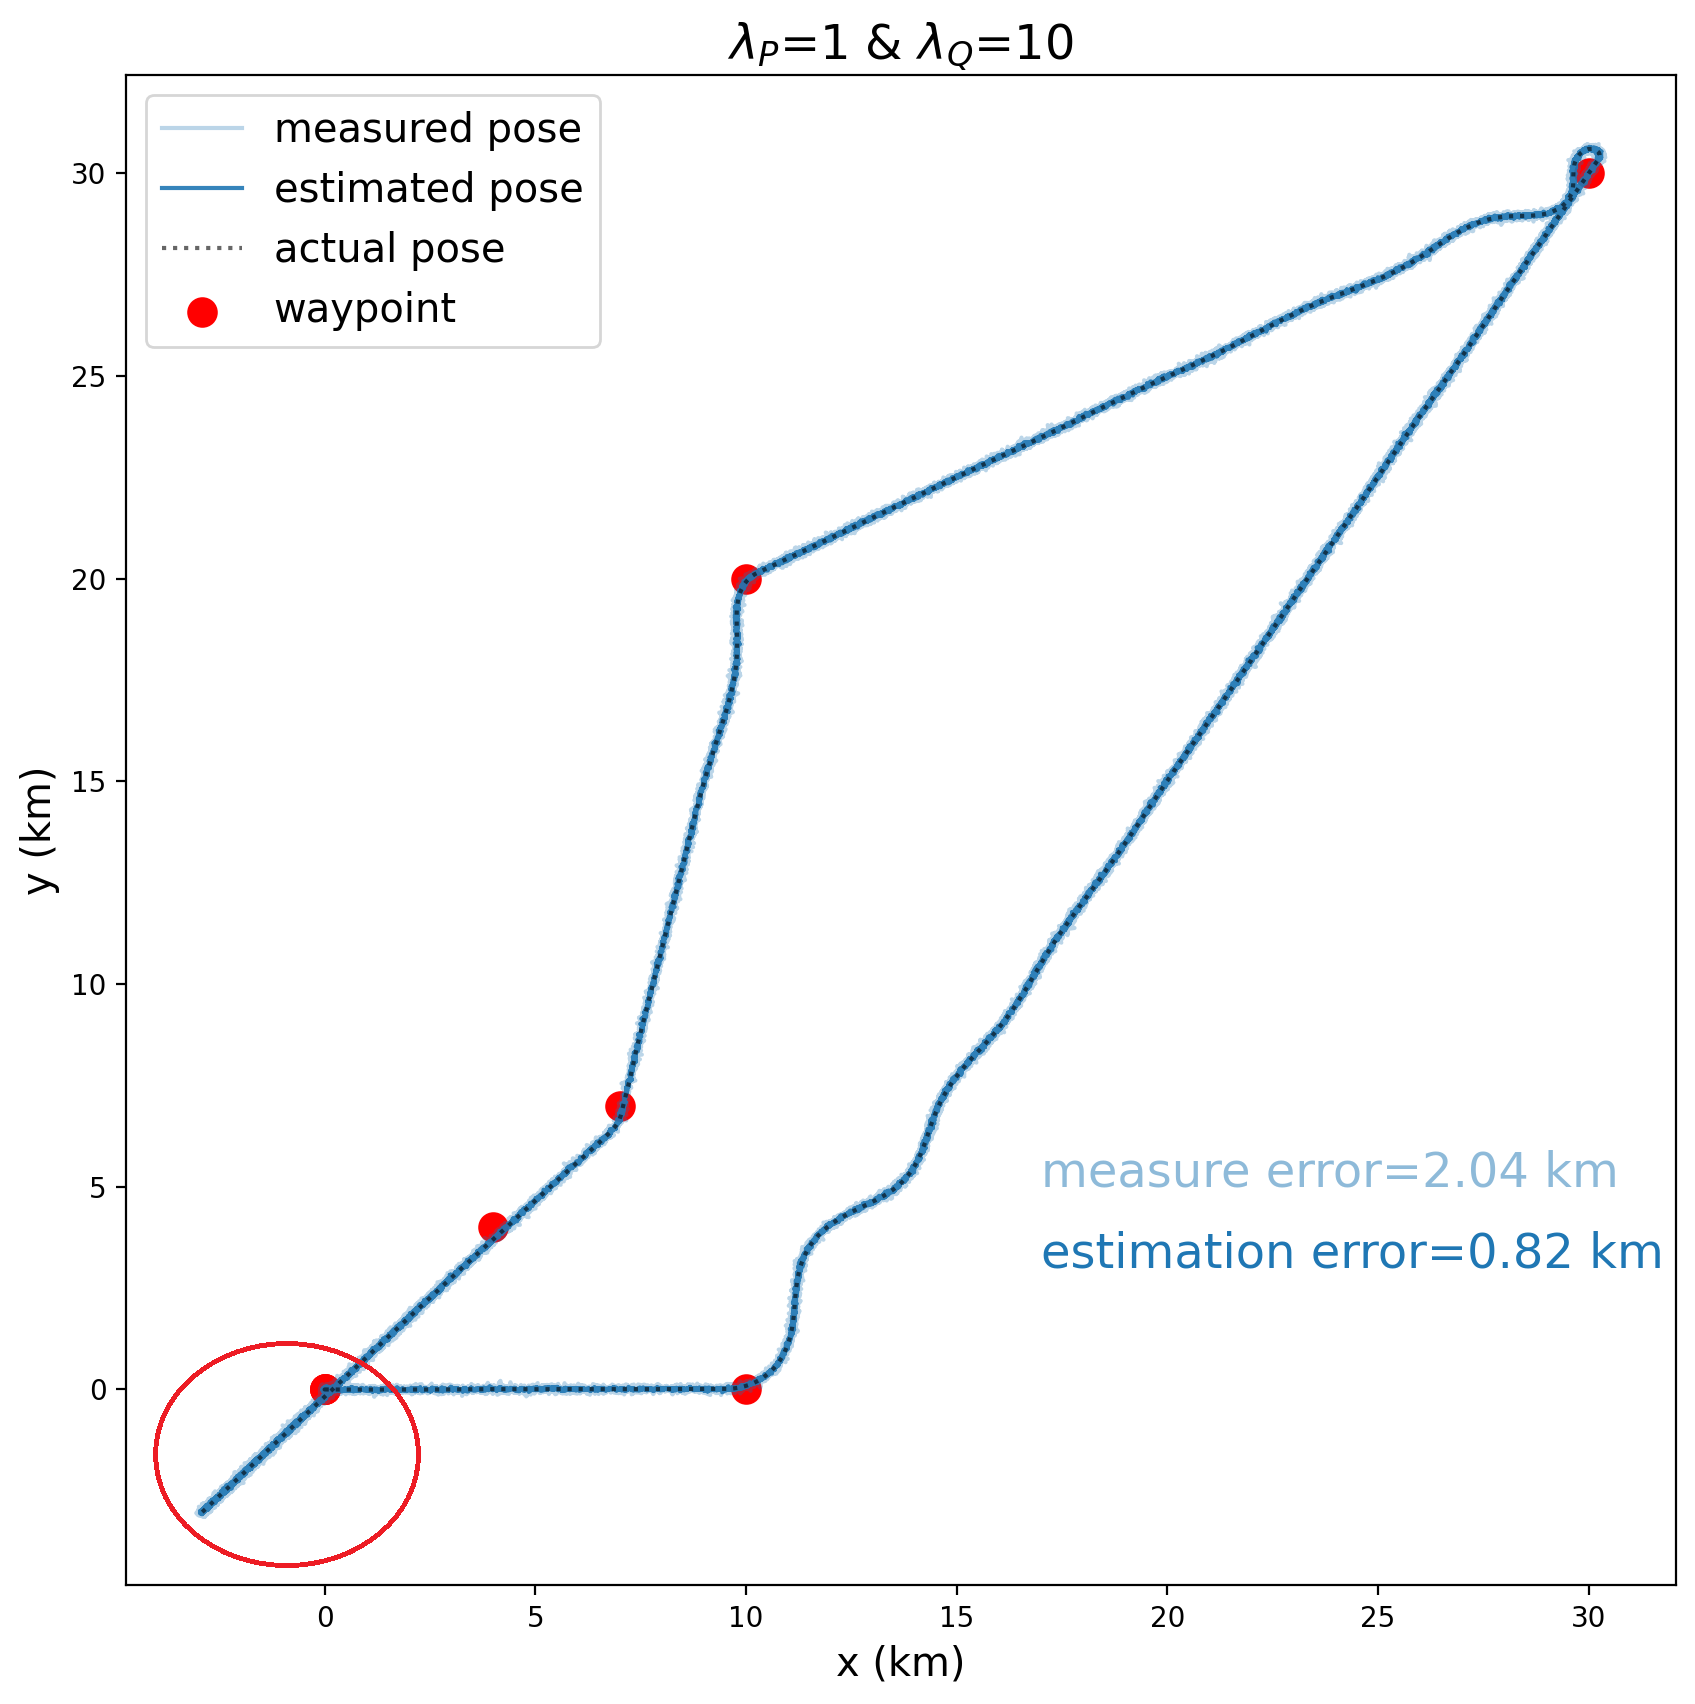
\includegraphics[width=\linewidth]{figures/estimate_P1_Q10_2d.png}
 		\caption{$\lambda_Q=1\:\&\:\lambda_R=10$}
 	\end{subfigure} 
 	\hfill
 	\begin{subfigure}[t]{0.24\textwidth}
 		\centering
 		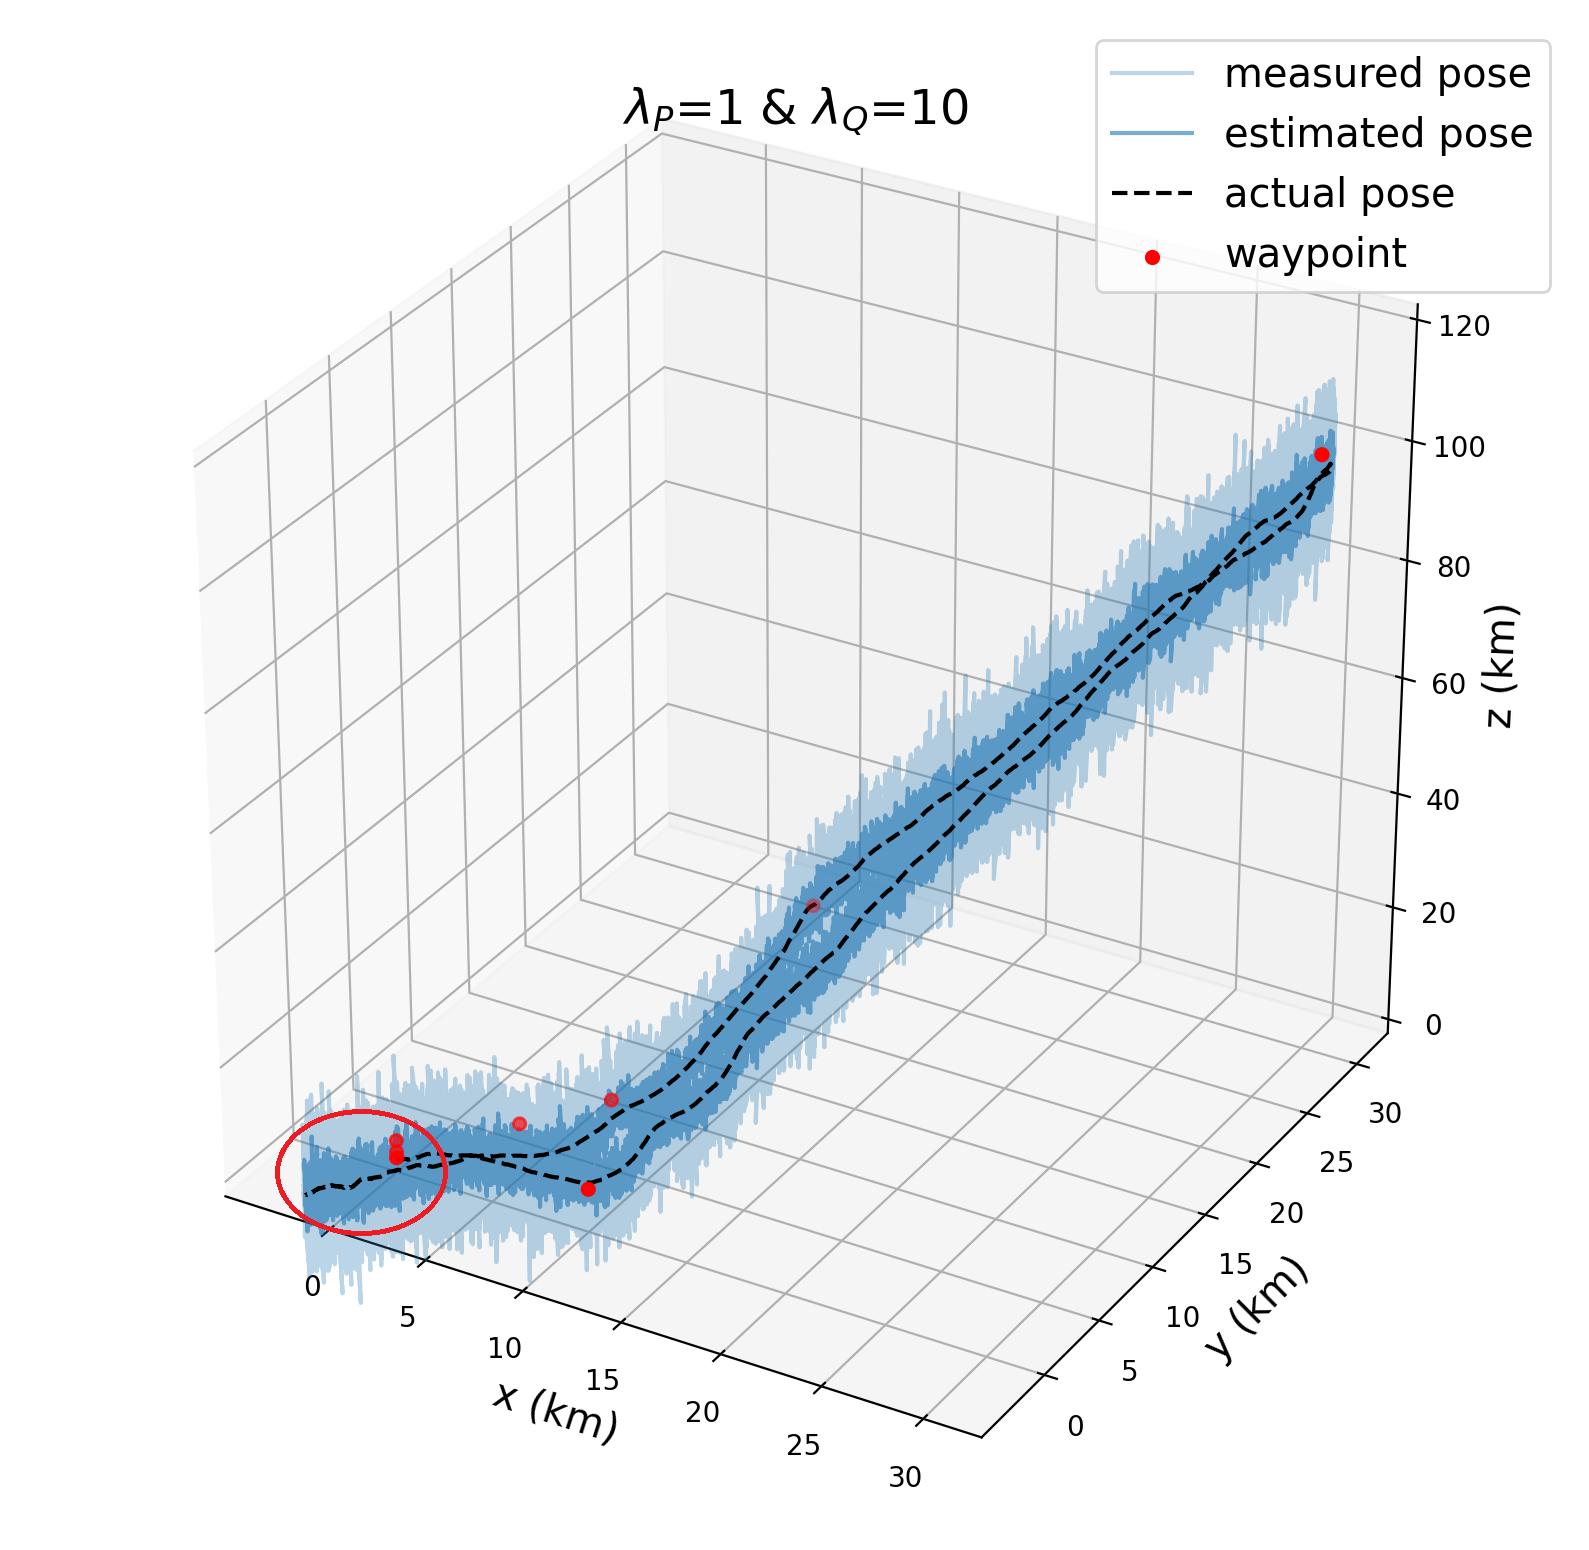
\includegraphics[width=\linewidth]{figures/estimate_P1_Q10_3d.png}
 		\caption{$\lambda_Q=1\:\&\:\lambda_R=10$}
 	\end{subfigure} \\
 	\hfill
 	\begin{subfigure}[t]{0.24\textwidth}
 		\centering
 		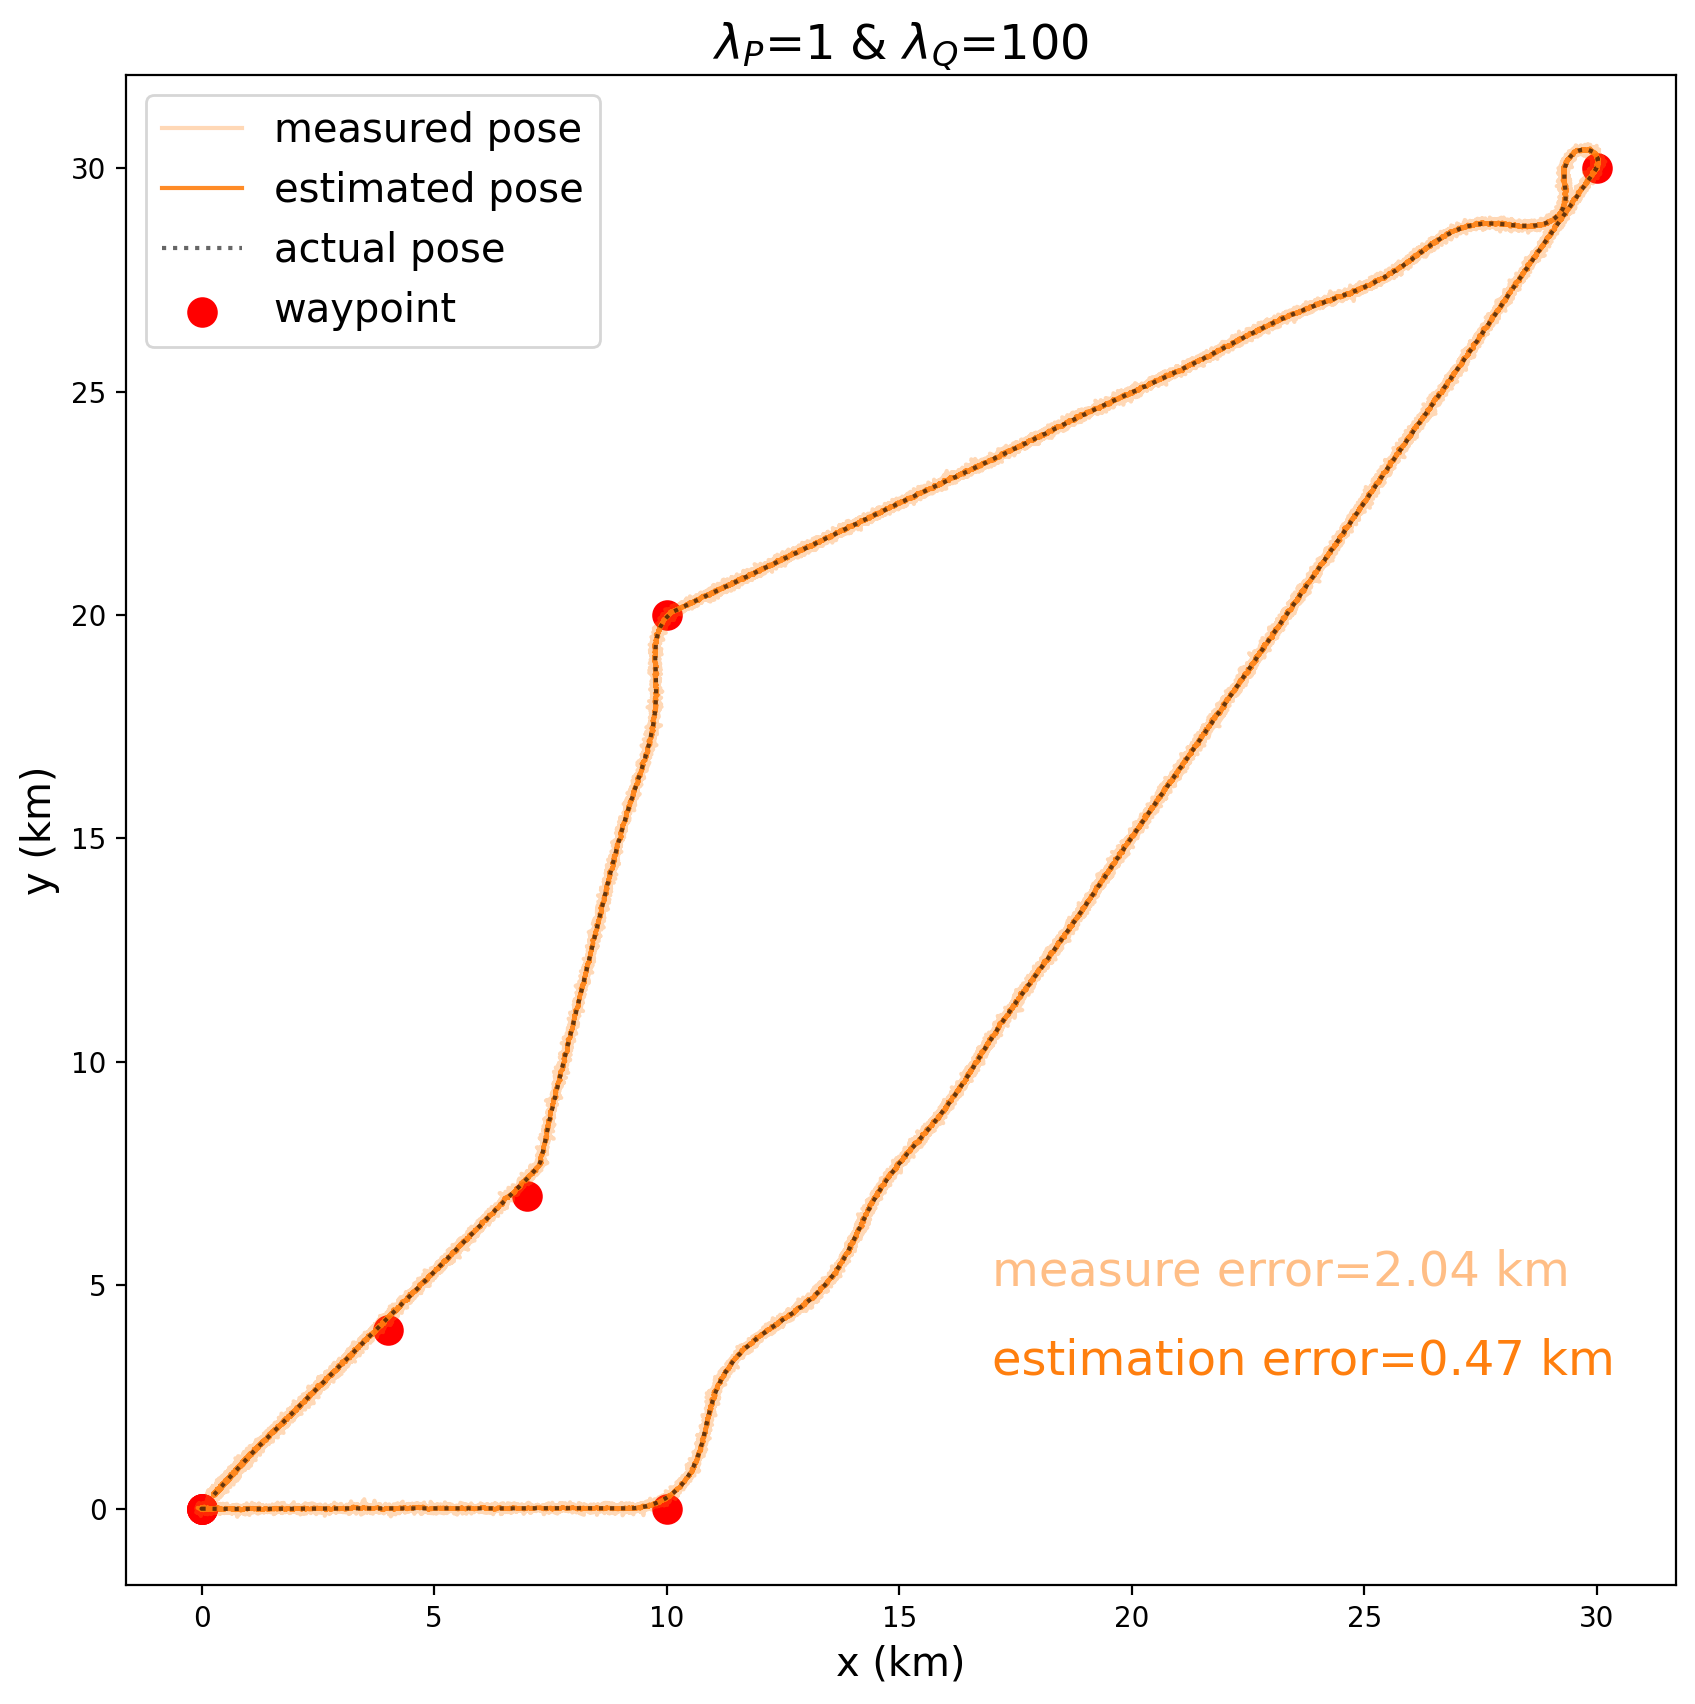
\includegraphics[width=\linewidth]{figures/estimate_P1_Q100_2d.png}
 		\caption{$\lambda_Q=1\:\&\:\lambda_R=10$}
 	\end{subfigure} 
 	\hfill
 	\begin{subfigure}[t]{0.24\textwidth}
 		\centering
 		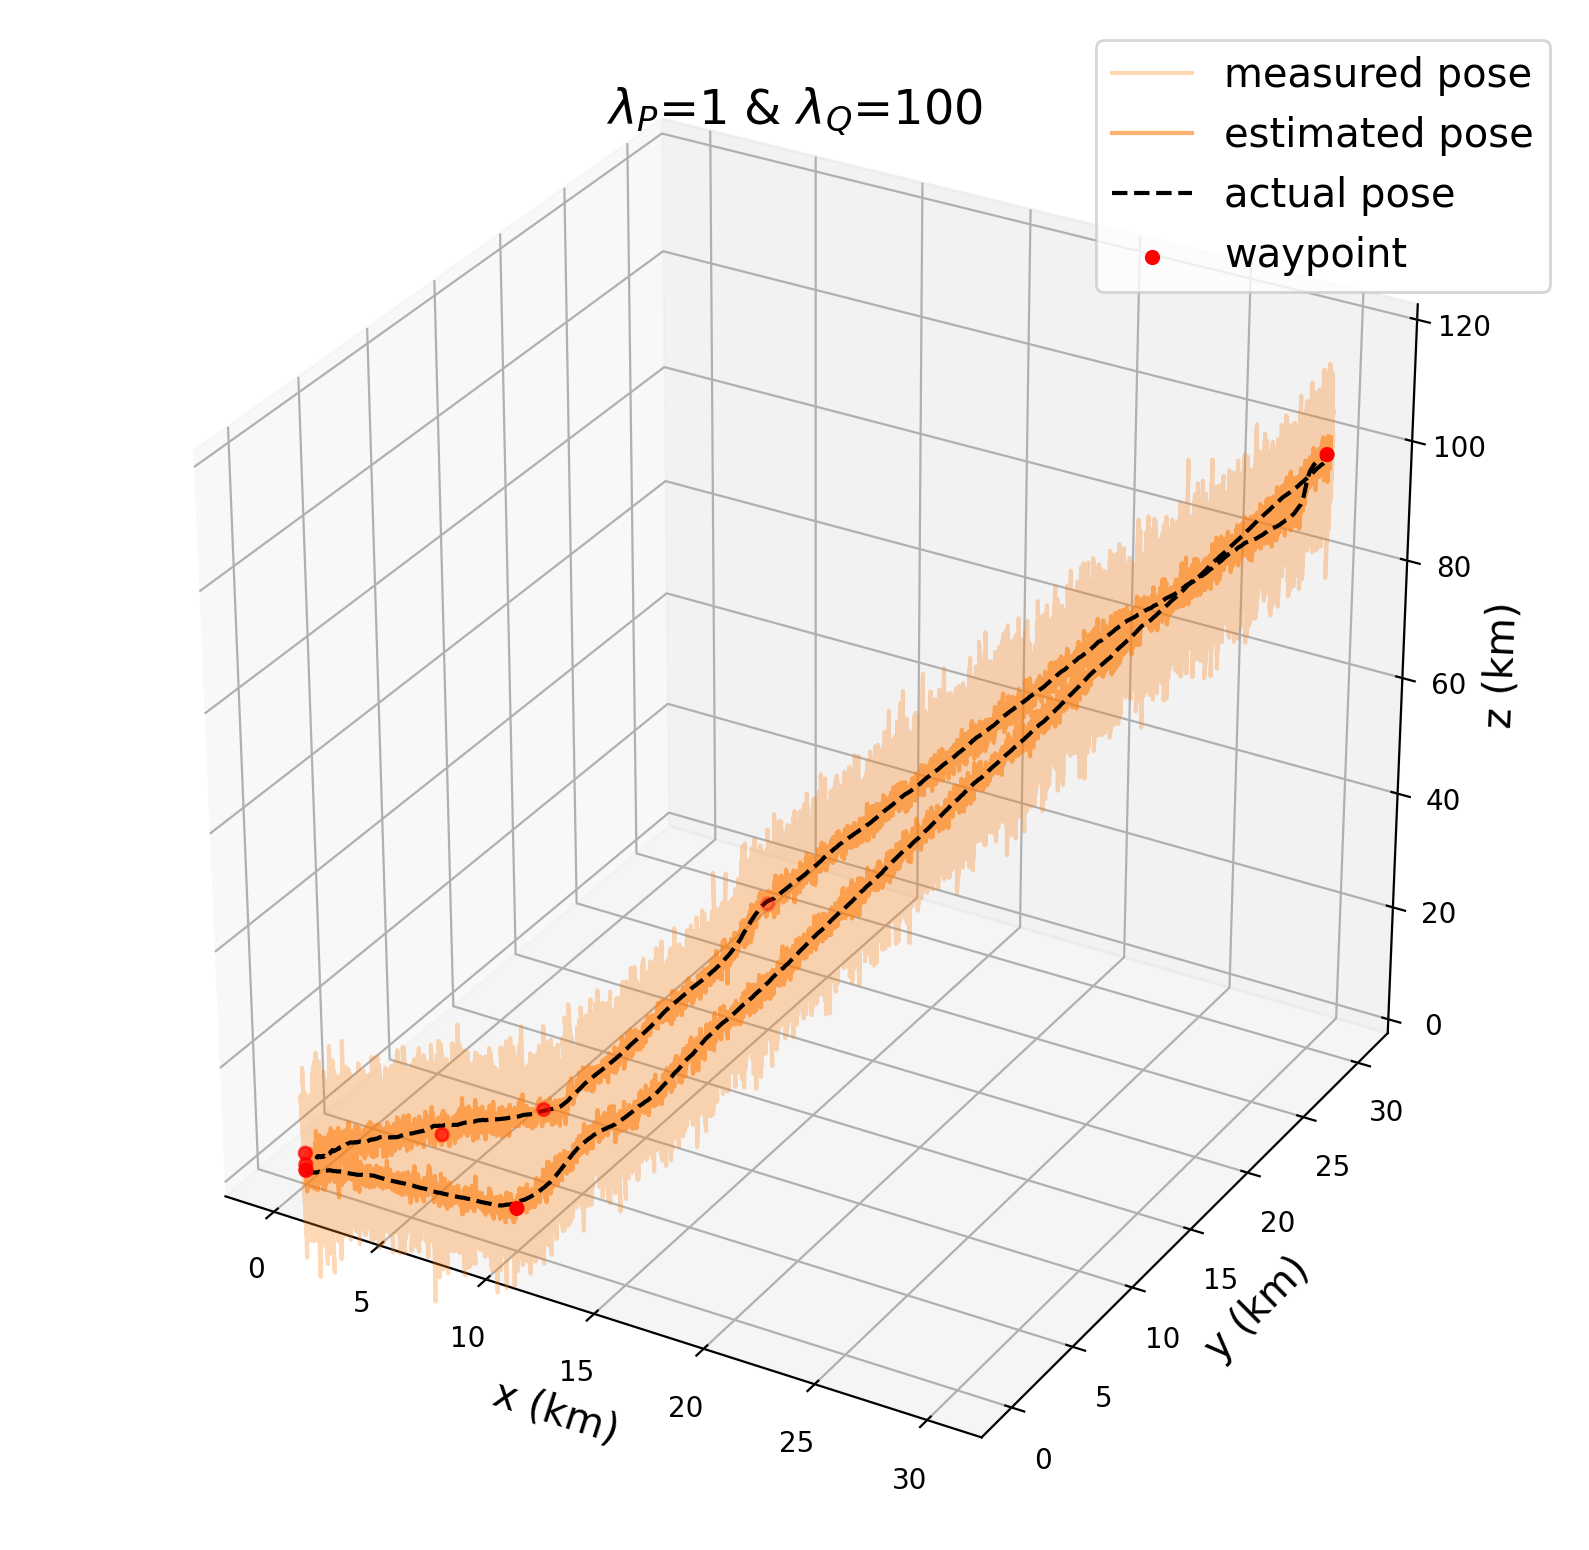
\includegraphics[width=\linewidth]{figures/estimate_P1_Q100_3d.png}
 		\caption{$\lambda_Q=1\:\&\:\lambda_R=10$}
 	\end{subfigure} \\
 	\hfill
 	\begin{subfigure}[t]{0.24\textwidth}
 		\centering
 		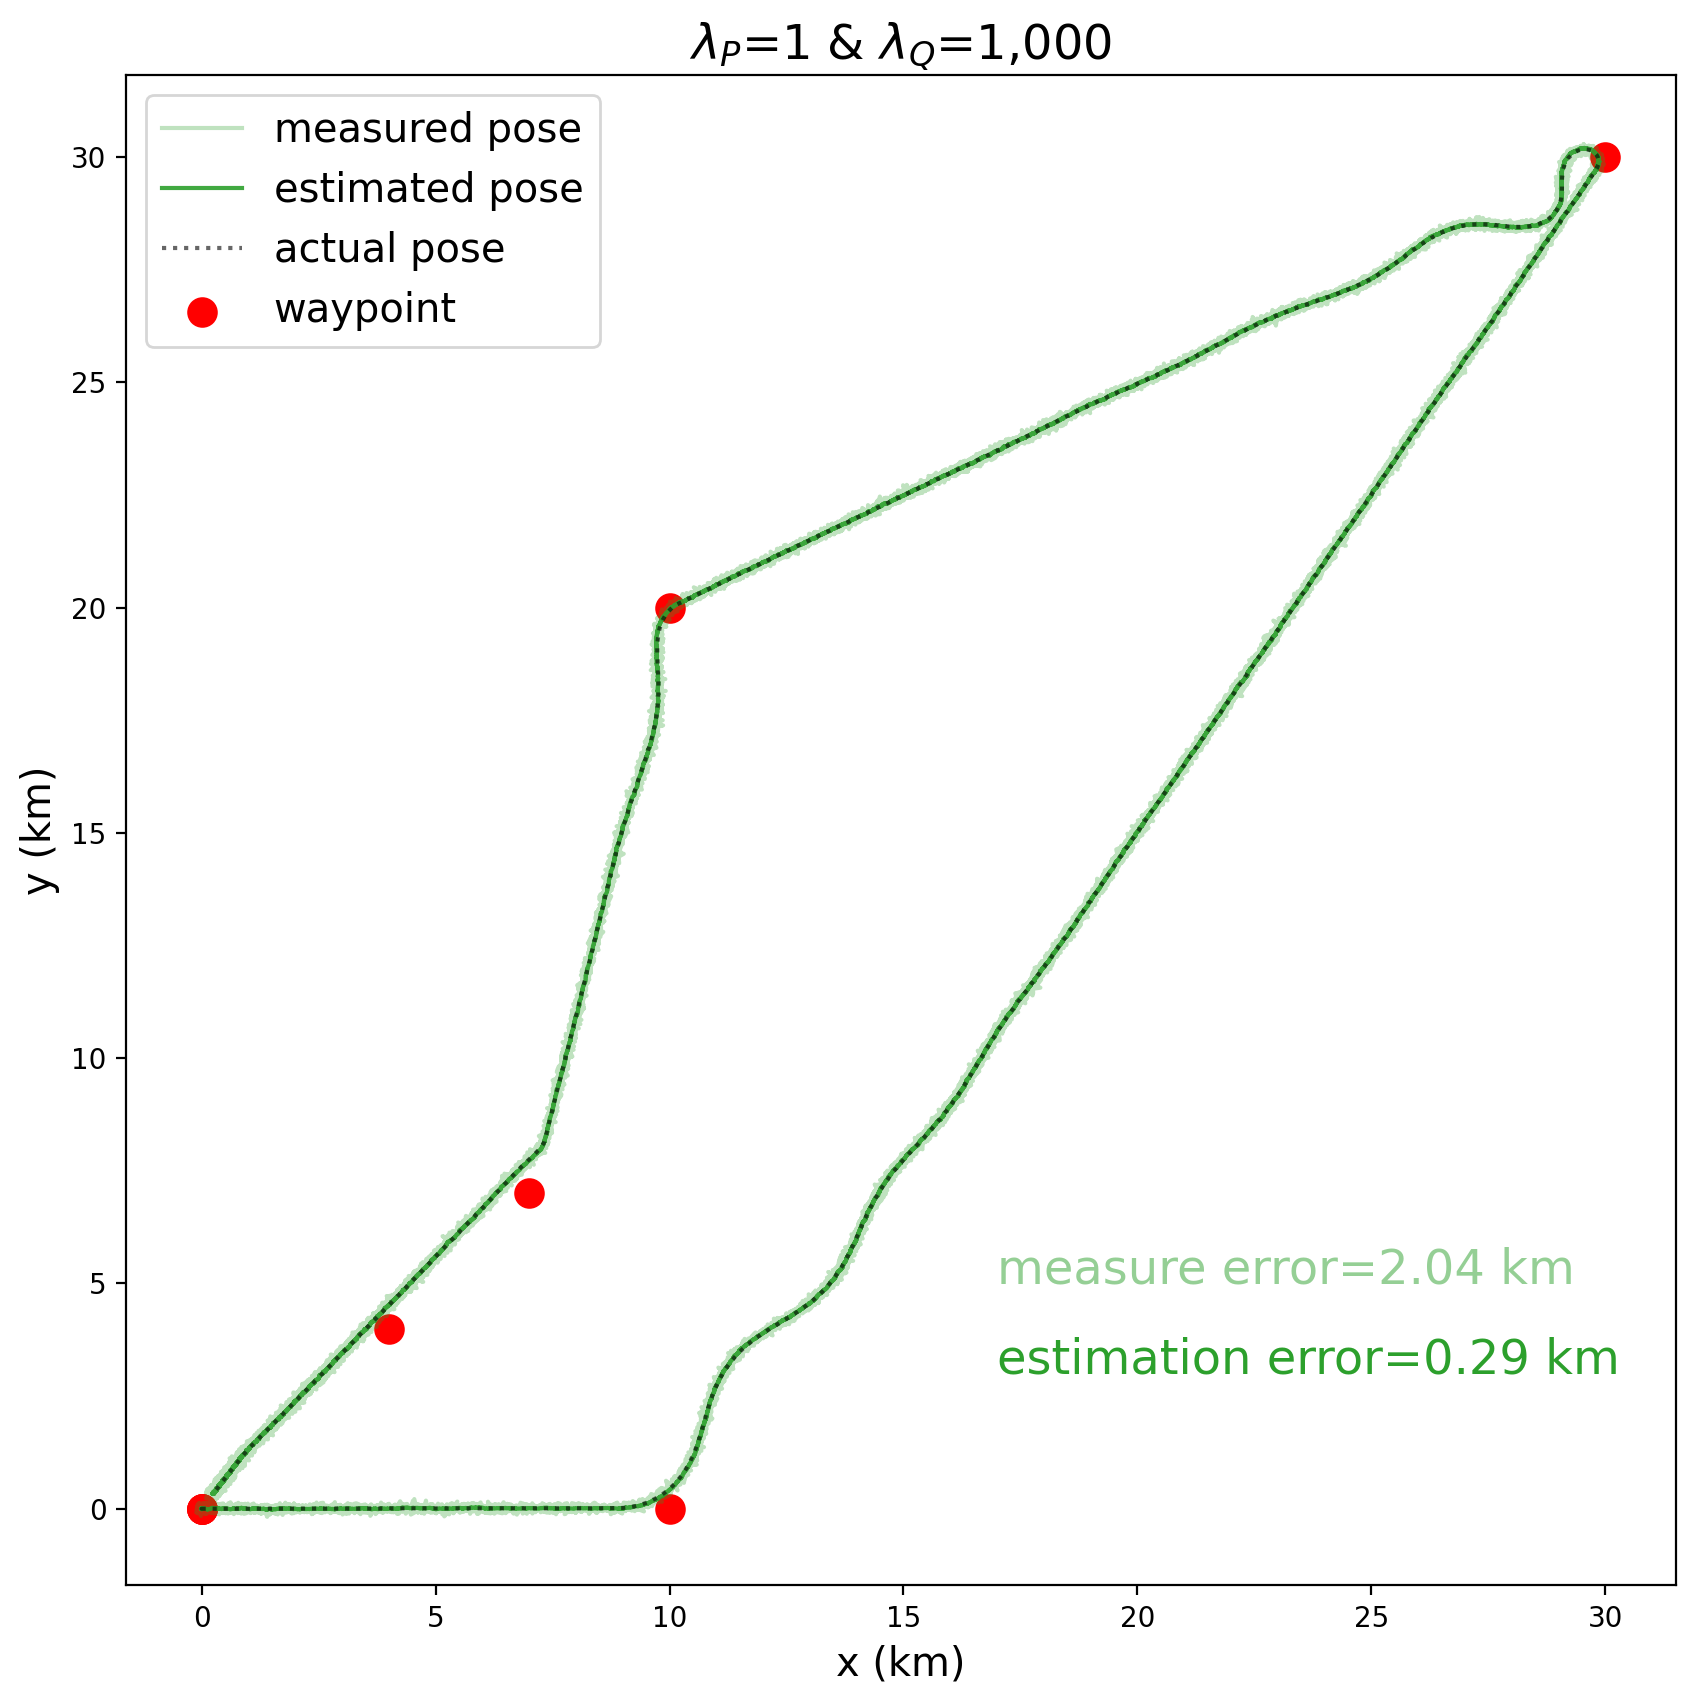
\includegraphics[width=\linewidth]{figures/estimate_P1_Q1000_2d.png}
 		\caption{$\lambda_Q=1\:\&\:\lambda_R=10$}
 	\end{subfigure} 
 	\hfill
 	\begin{subfigure}[t]{0.24\textwidth}
 		\centering
 		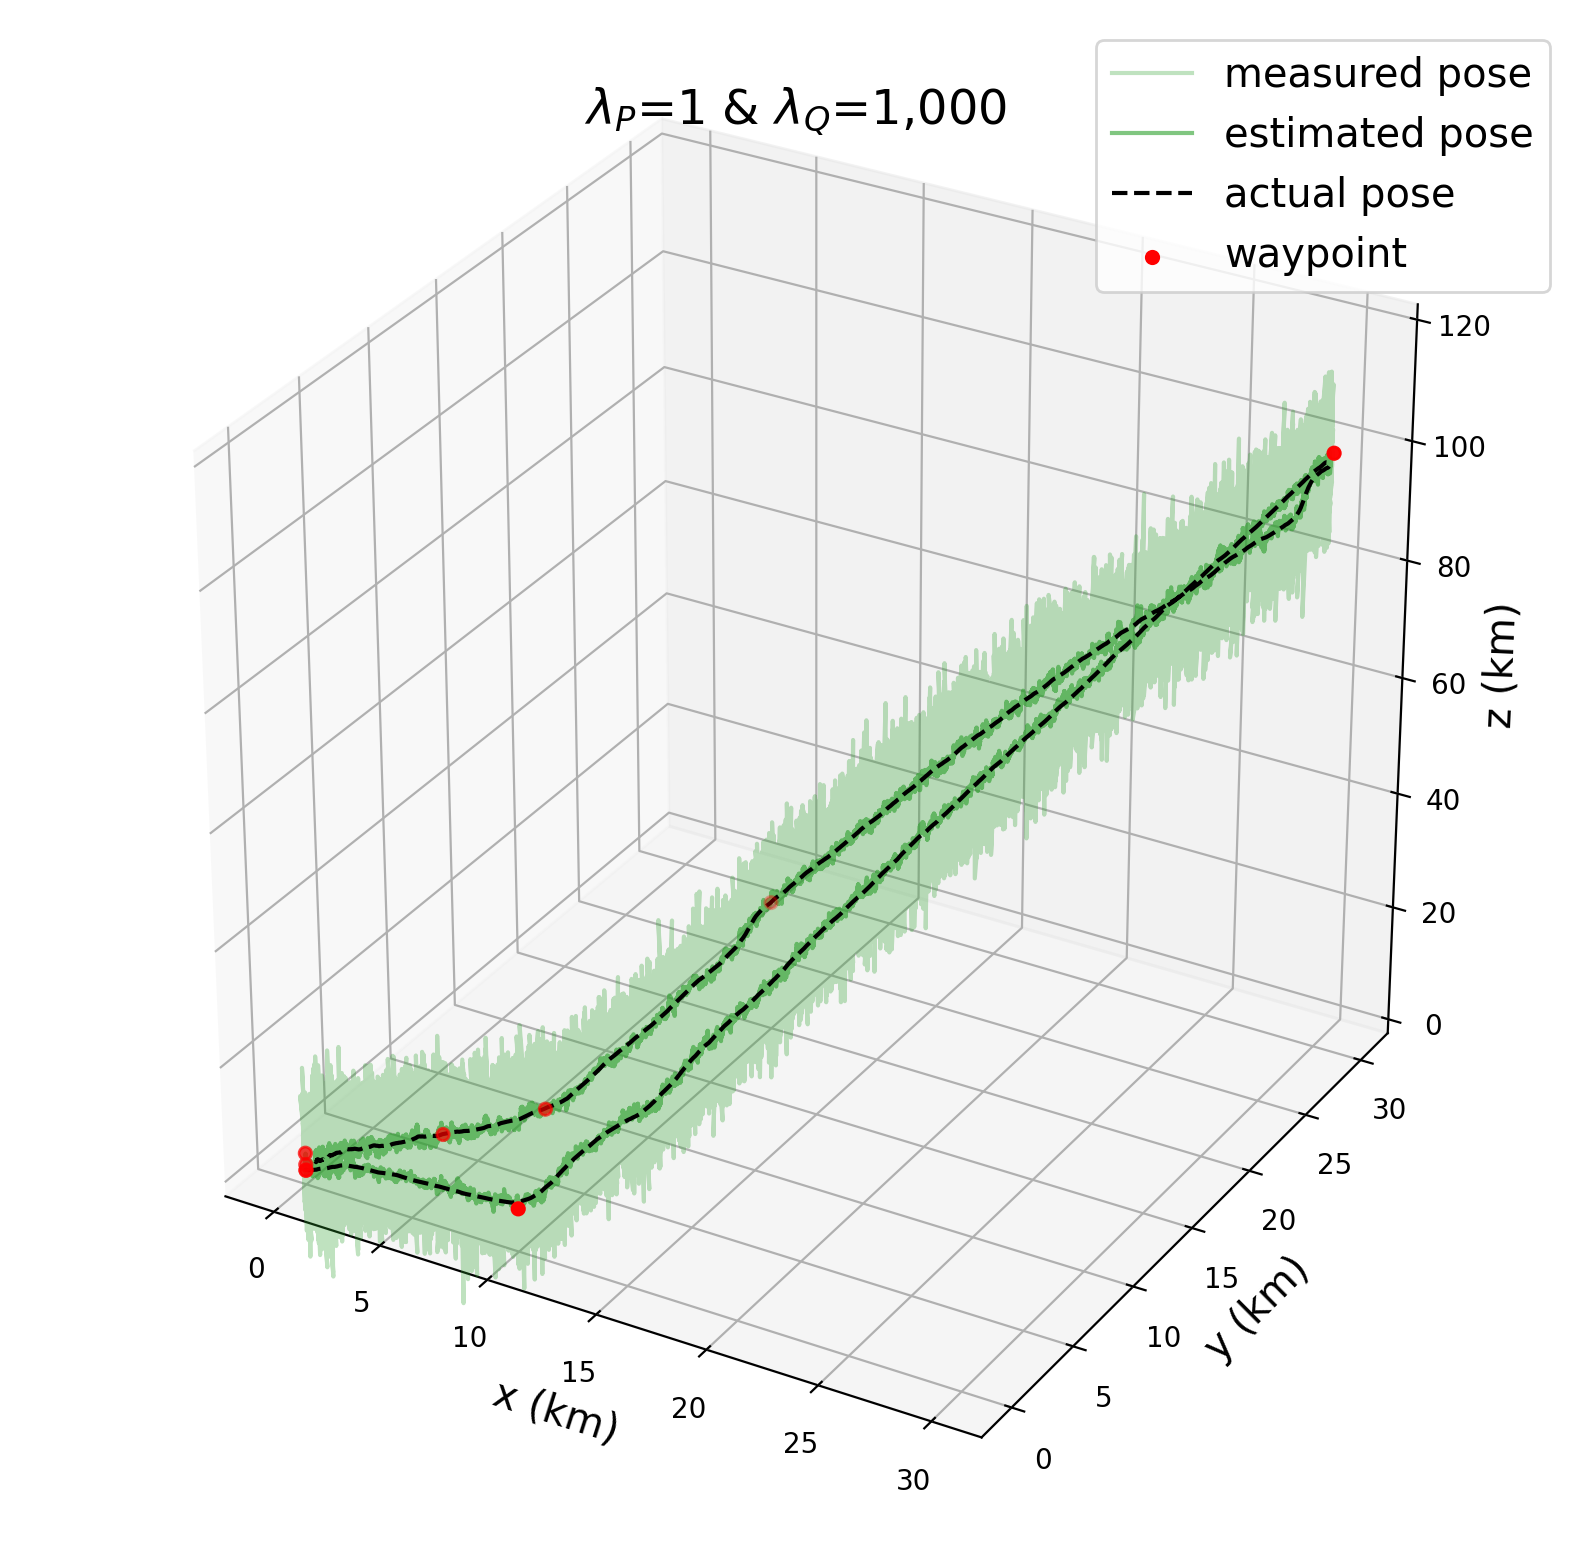
\includegraphics[width=\linewidth]{figures/estimate_P1_Q1000_3d.png}
 		\caption{$\lambda_Q=1\:\&\:\lambda_R=10$}
 	\end{subfigure} 
 	
 	\caption{Two-dimensional plot (left column: a, c, and e) and three-dimensional plot (right column: b, d, and f) of the measured trajectories and the estimated trajectories with $\lambda_Q=1\:\&\:\lambda_R=10$ (blue), $\lambda_Q=1\:\&\:\lambda_R=100$ (orange), and $\lambda_Q=1\:\&\:\lambda_R=1,000$ (green).}
 	
 	\label{fig:exp_QR}
 \end{figure}
  
 The result of the first experiment is shown in Fig.~\ref{fig:exp_QR}. The figure presents that, due to a strong measurement noise, using large $\lambda_R$ improves the estimation performance. Without state estimation, the root-mean-square error of the measured trajectory is 2.04 km in all cases. Using $\lambda_Q=1\:\&\:\lambda_R=1,000$ can lower the root-mean-square error to 0.29 km (i.e., 86\% reduction). Interestingly, if $\lambda_Q=1\:\&\:\lambda_R=1,000$, the error is relatively high, or rather 0.82. Consequently, the spaceship misses the acceptance sphere and does not stop at stopping point, as highlighted by red circles in Fig.~\ref{fig:exp_QR}(a,b). 
 

\subsection{Experiment 2: Control}
\label{sec:exp_control}

With $\lambda_Q=1\:\&\:\lambda_R=1,000$, the second experiment compares three values $K_d$. Those are $K_d=500$ (blue), $K_d=1,000$ (orange), and $K_d=1,500$ (green). Note that, in this experiment, $K_p$ representing convergence time is fixed as 1,000 during the comparison. increasing $K_p$ will increase the speed of the spaceship.  During this, the guidance parameter $\eta_\Delta$ and $\eta_e$ are still fixed at 100 and 0.1.

\begin{figure}[h]
	\centering
	\begin{subfigure}[t]{0.24\textwidth}
		\centering
		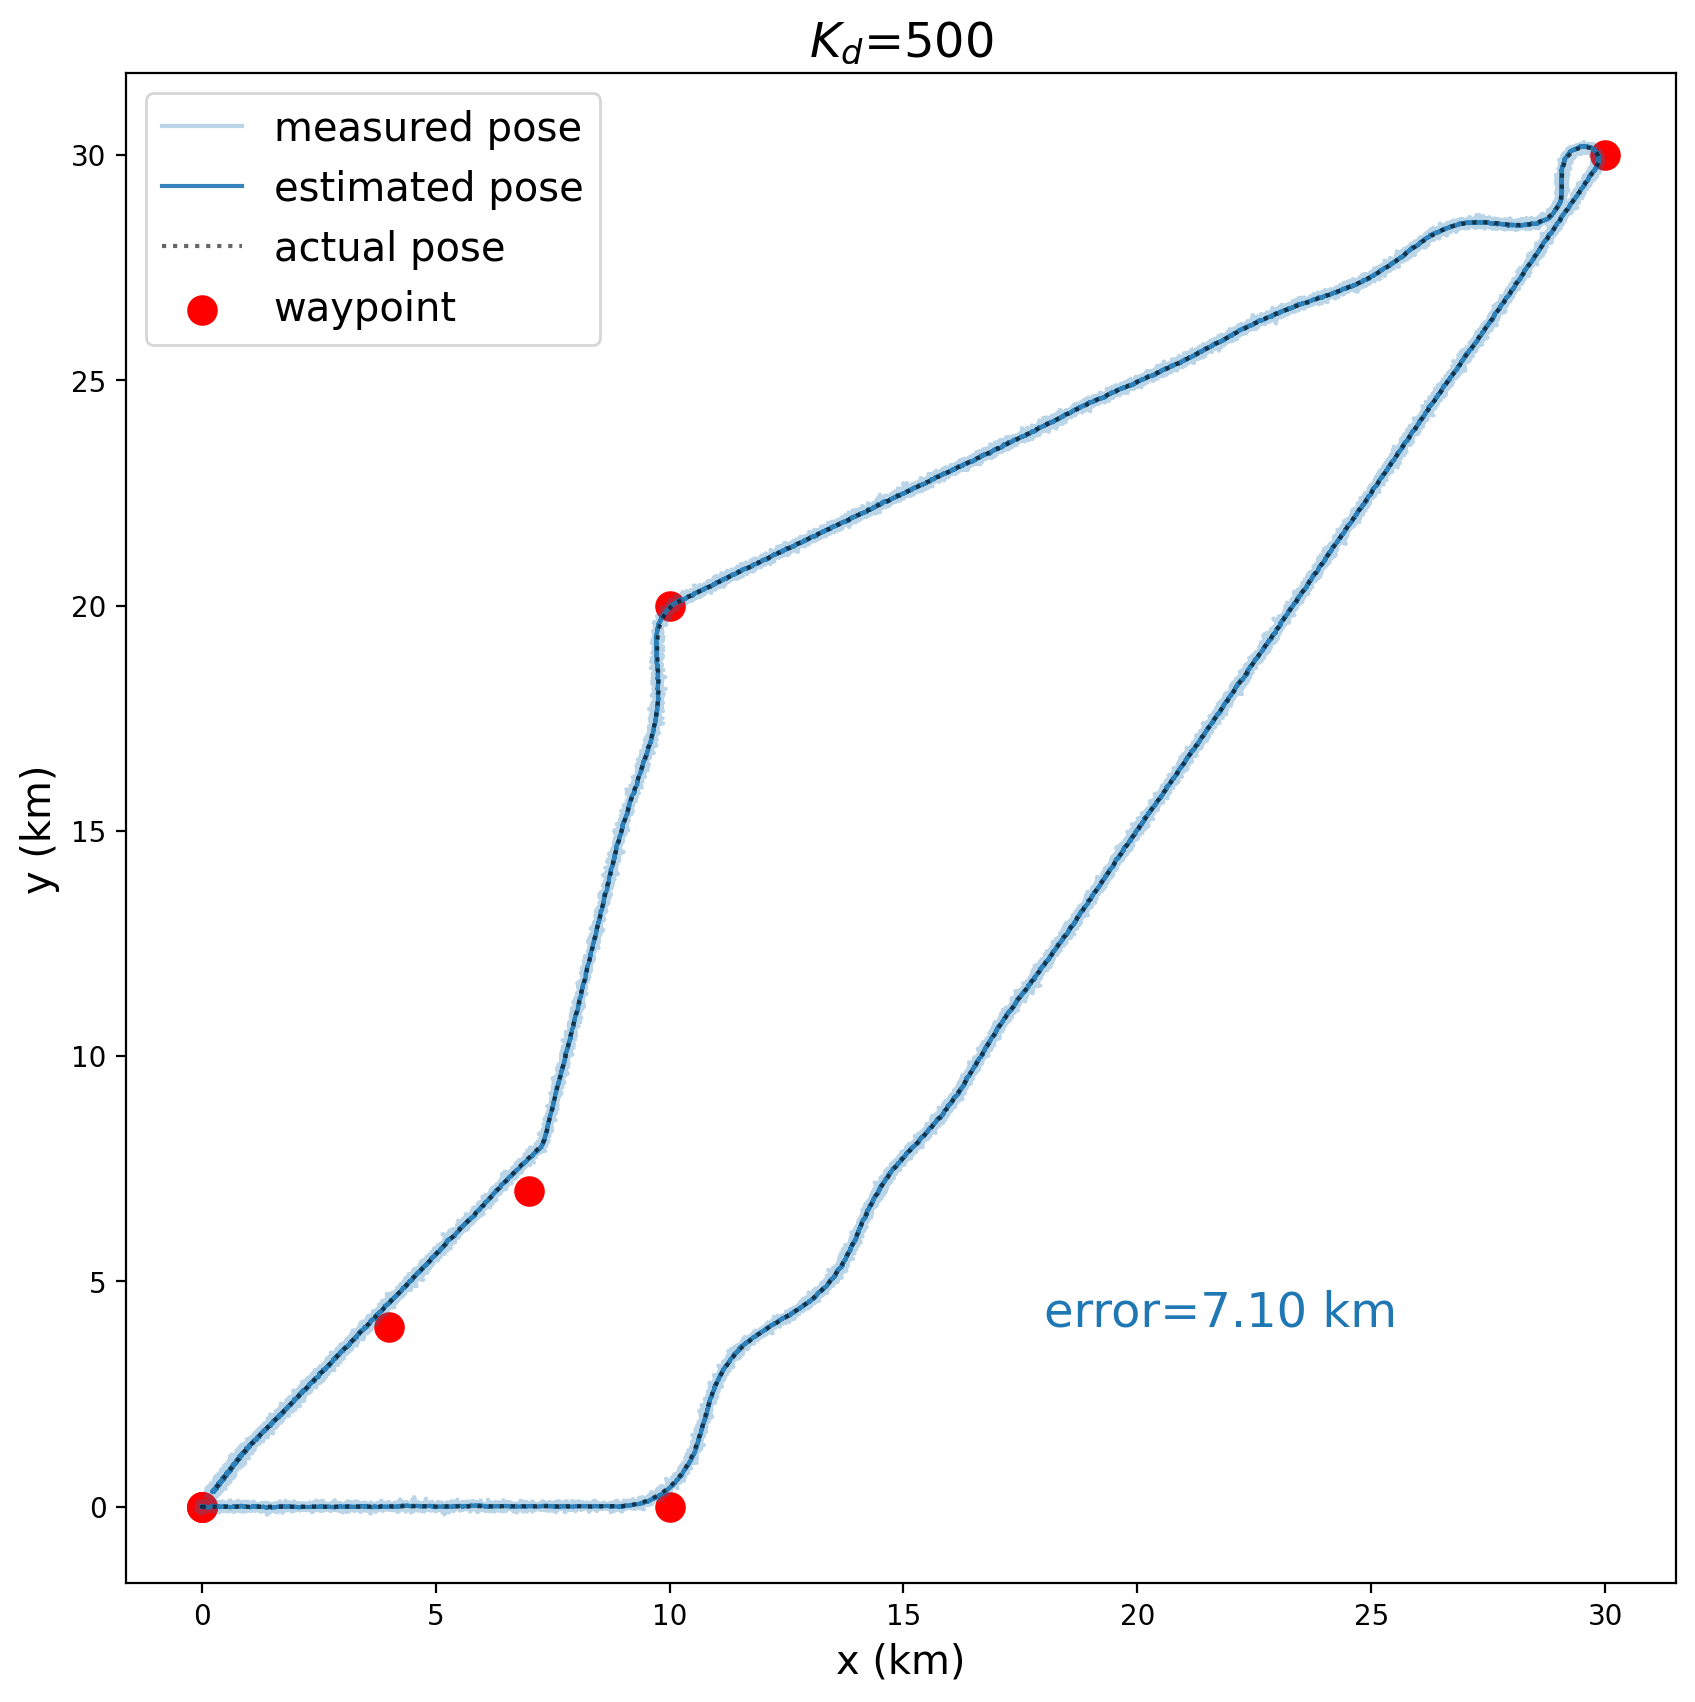
\includegraphics[width=\linewidth]{figures/Dgain_D05_2d.png}
		\caption{$K_d=500$}
	\end{subfigure} 
	\hfill
	\begin{subfigure}[t]{0.24\textwidth}
		\centering
		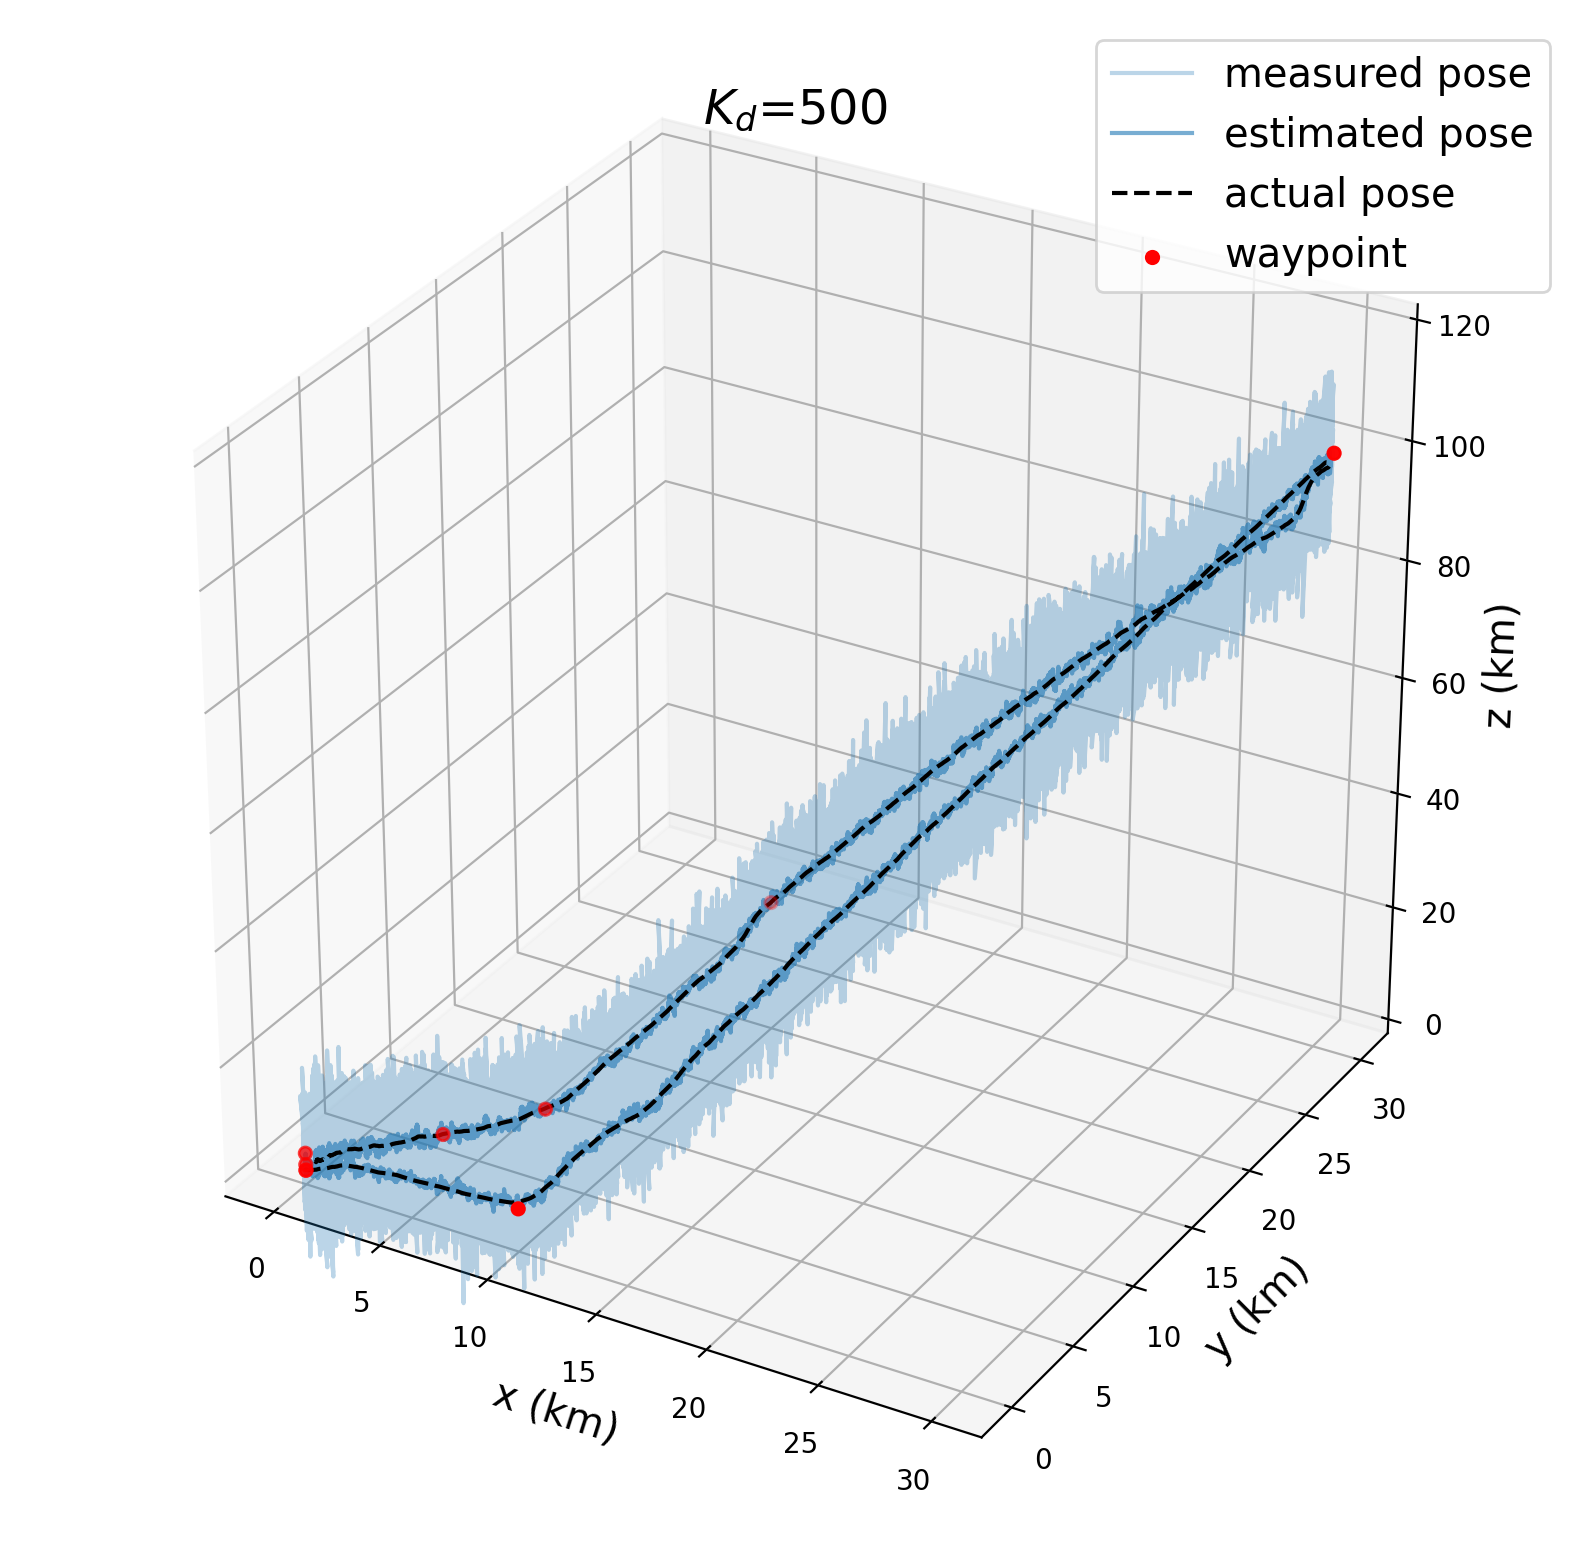
\includegraphics[width=\linewidth]{figures/Dgain_D05_3d.png}
		\caption{$K_d=500$}
	\end{subfigure} \\
	\hfill
	\begin{subfigure}[t]{0.24\textwidth}
		\centering
		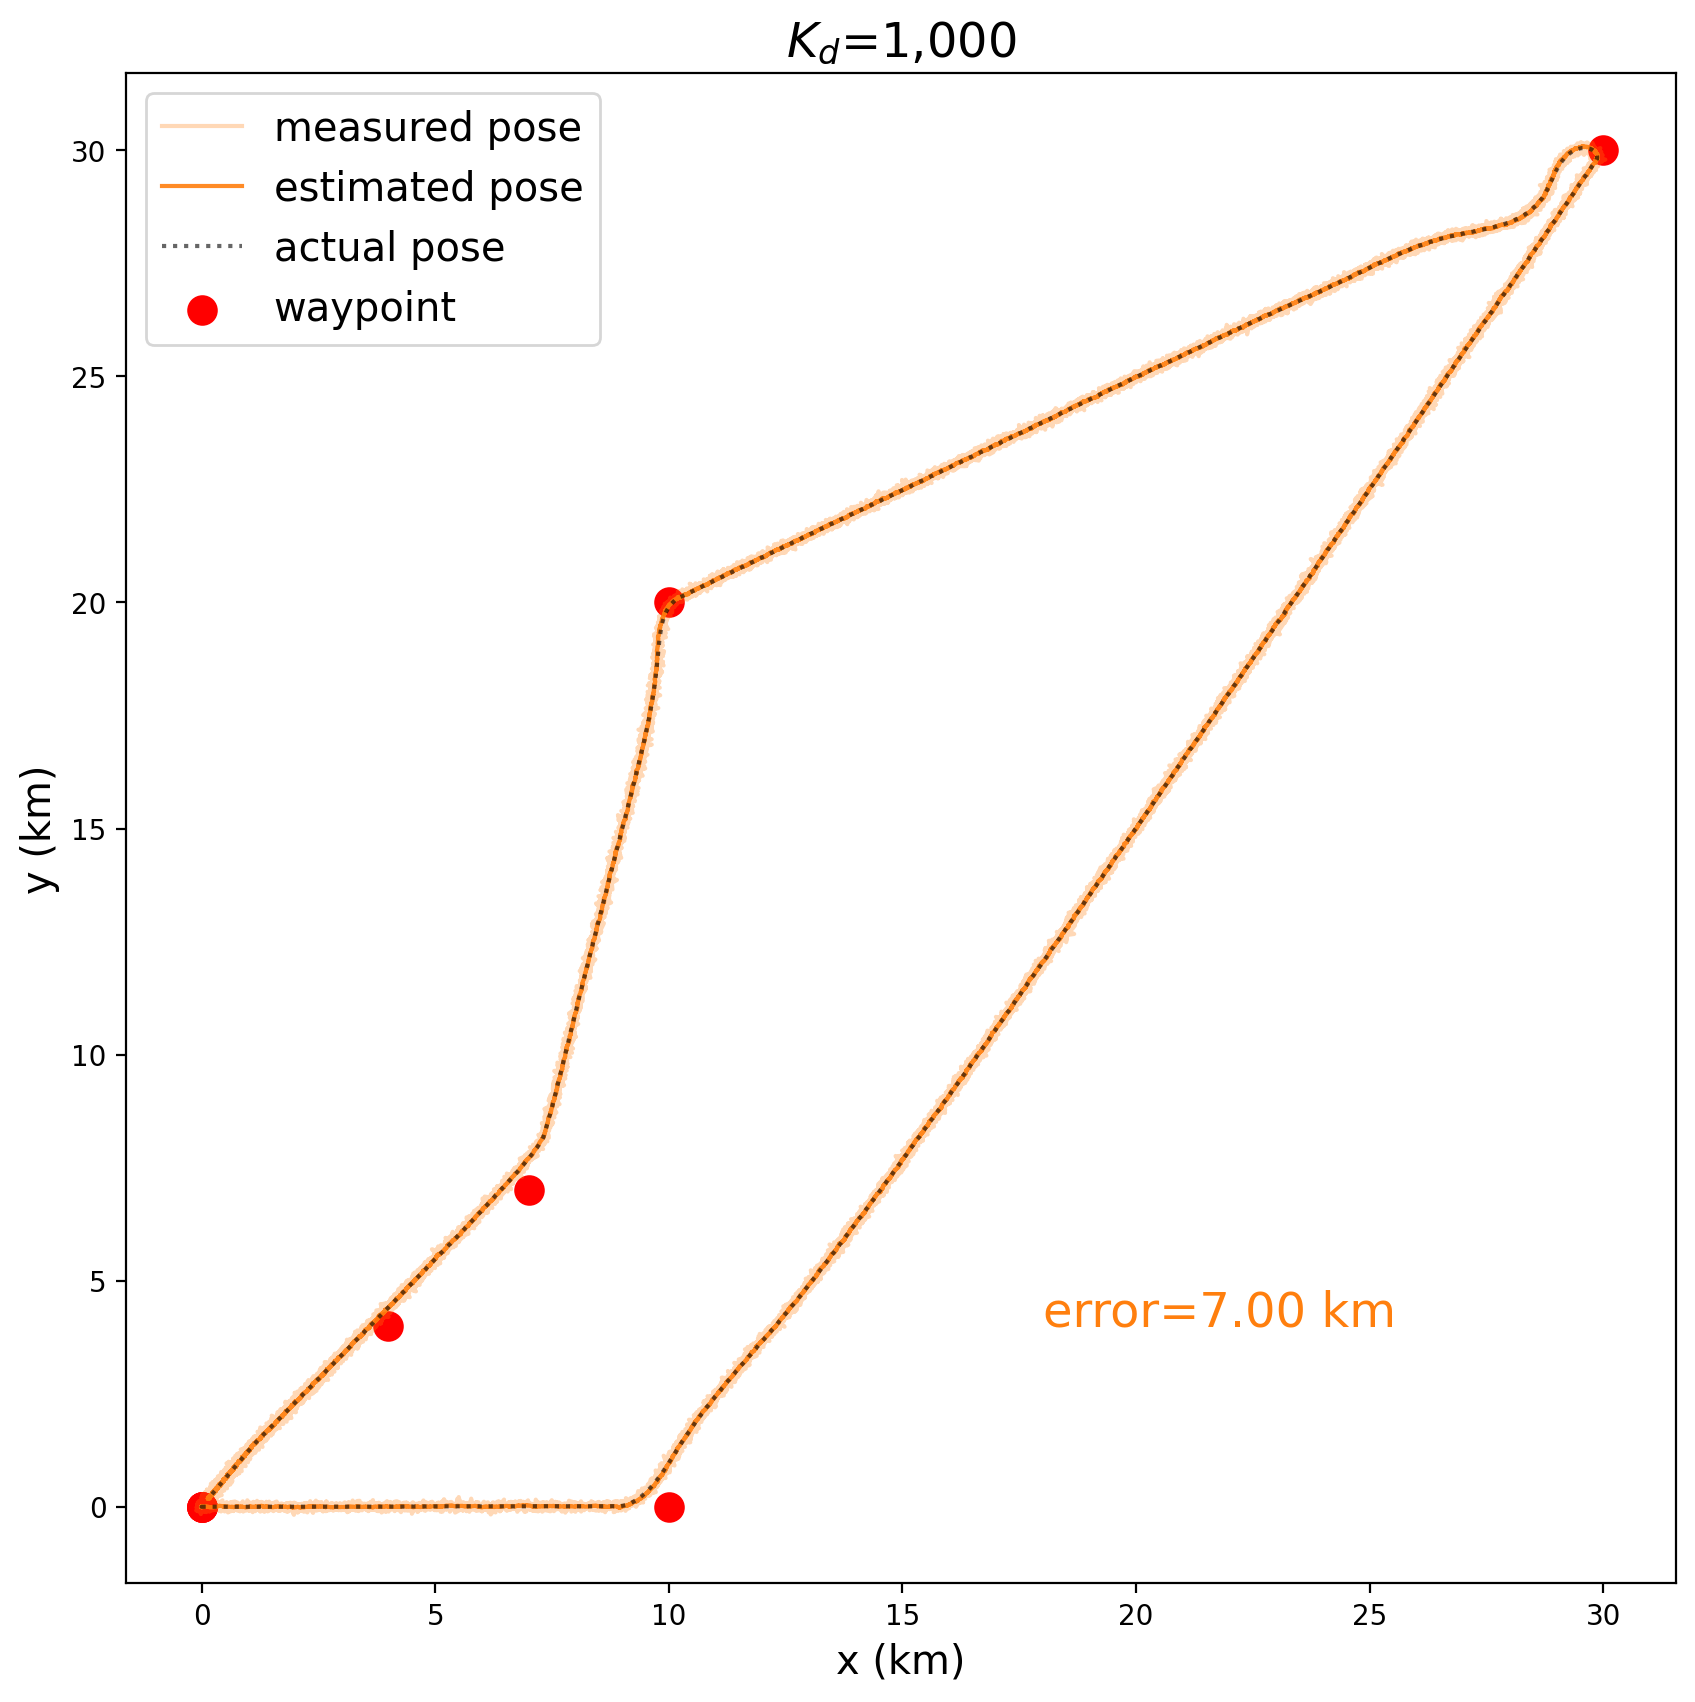
\includegraphics[width=\linewidth]{figures/Dgain_D10_2d.png}
		\caption{$K_d=100$}
	\end{subfigure} 
	\hfill
	\begin{subfigure}[t]{0.24\textwidth}
		\centering
		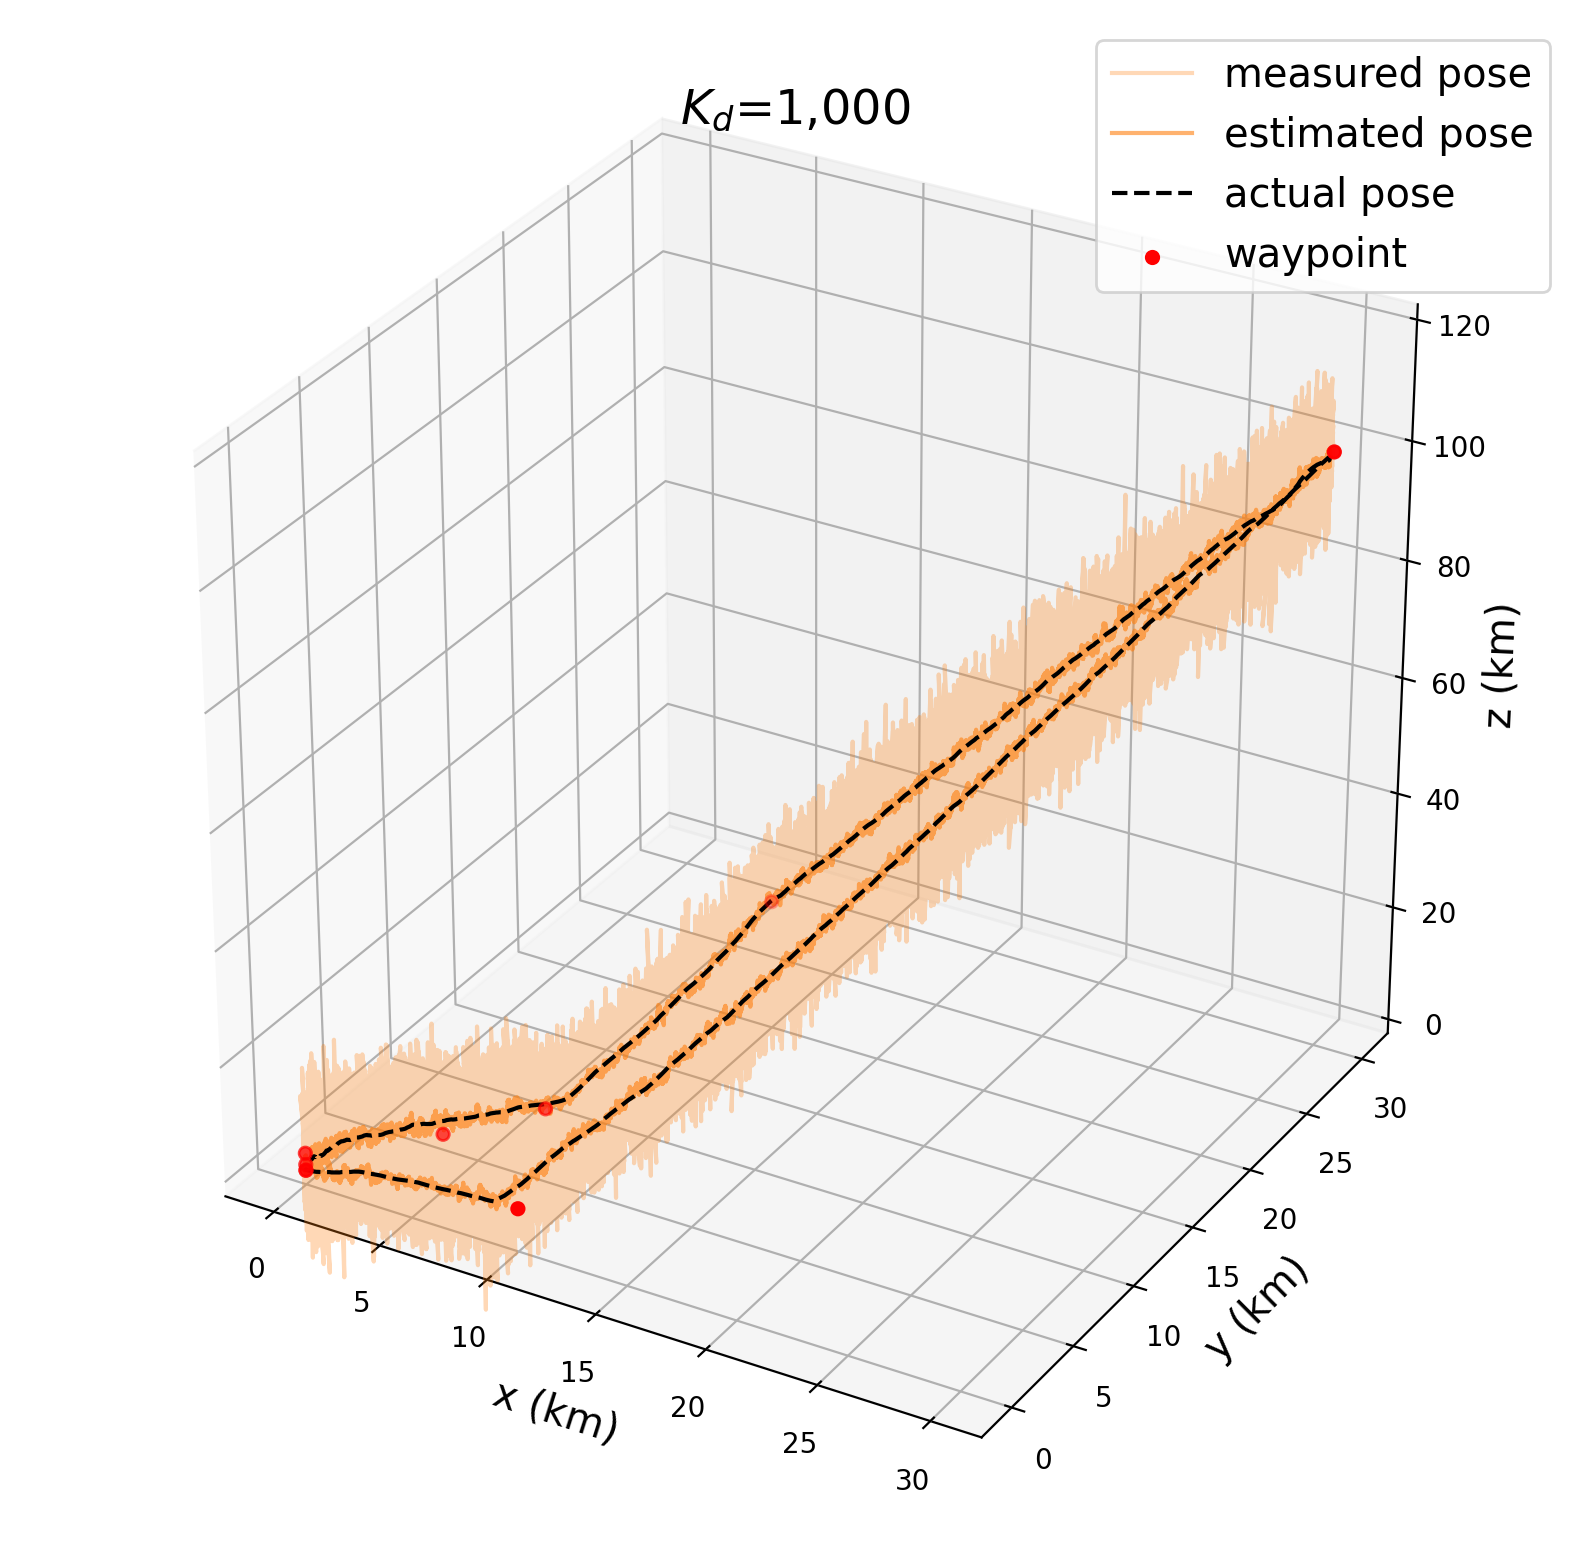
\includegraphics[width=\linewidth]{figures/Dgain_D10_3d.png}
		\caption{$K_d=100$}
	\end{subfigure} \\
	\hfill
	\begin{subfigure}[t]{0.24\textwidth}
		\centering
		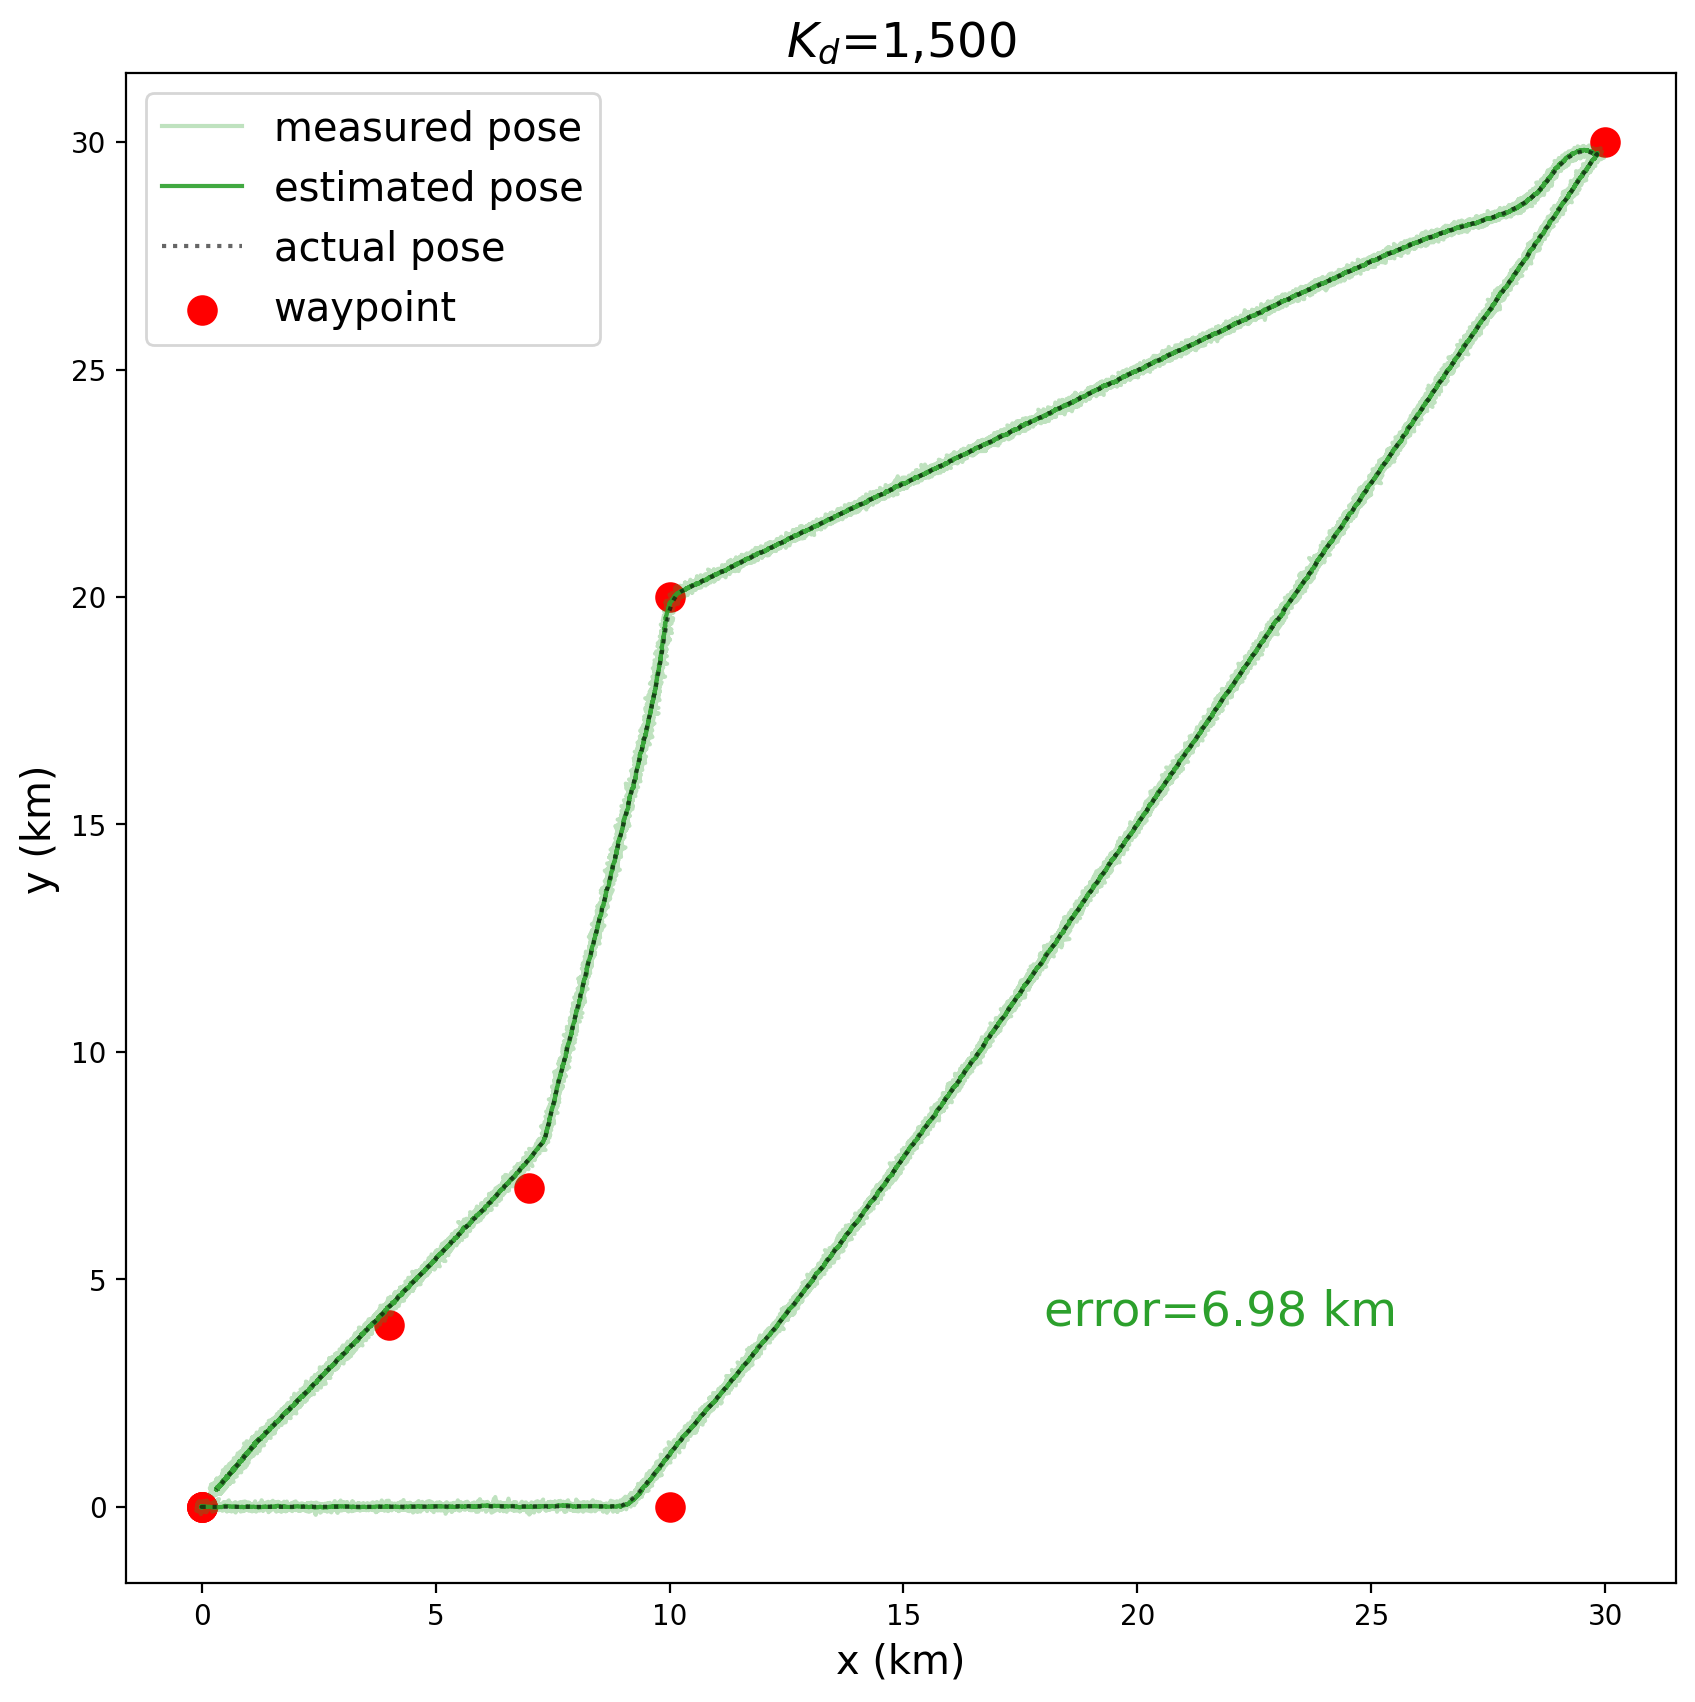
\includegraphics[width=\linewidth]{figures/Dgain_D15_2d.png}
		\caption{$K_d=1,500$}
	\end{subfigure} 
	\hfill
	\begin{subfigure}[t]{0.24\textwidth}
		\centering
		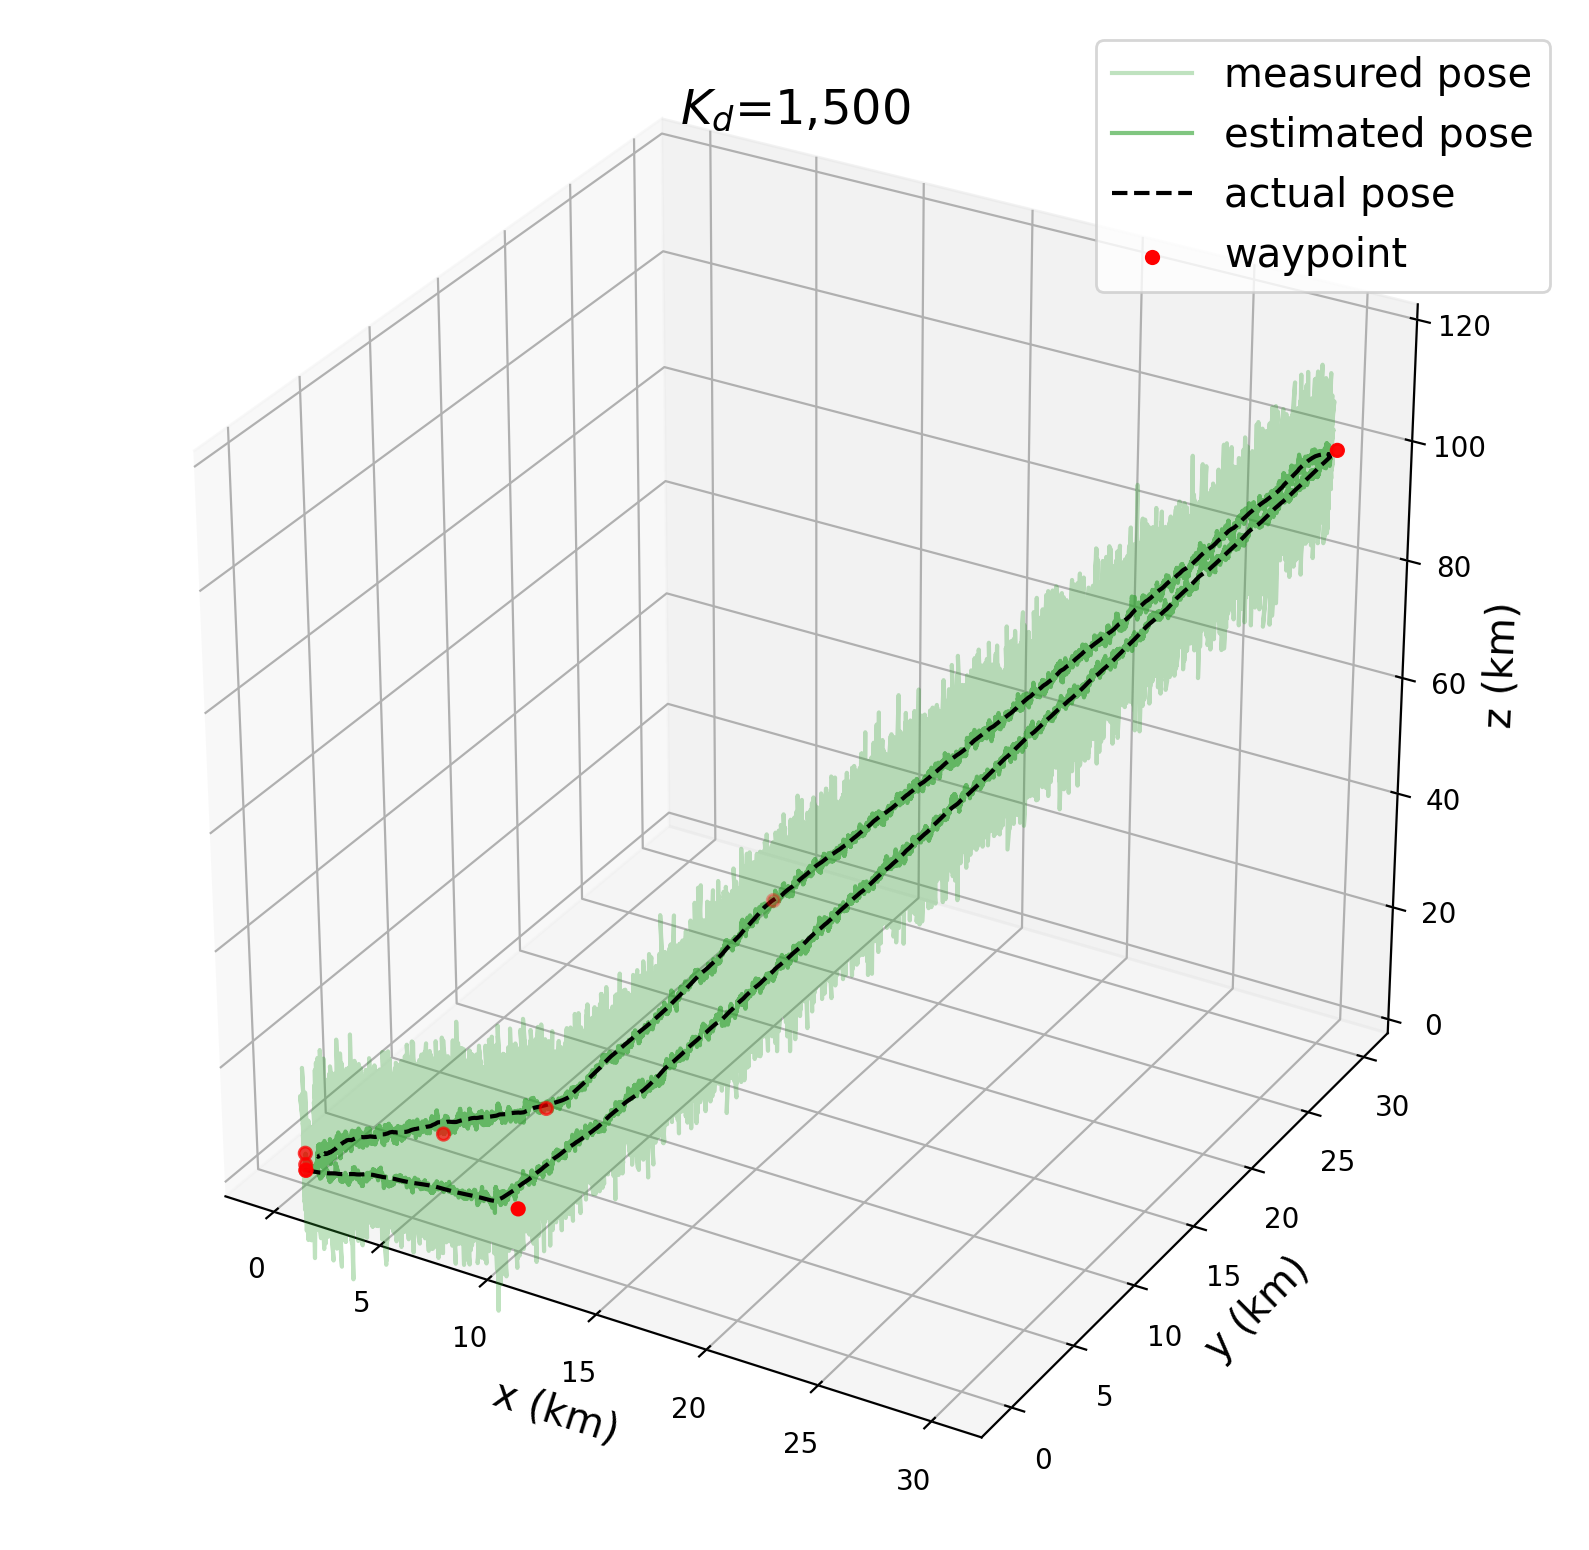
\includegraphics[width=\linewidth]{figures/Dgain_D15_3d.png}
		\caption{$K_d=1,500$}
	\end{subfigure} 
	
	\caption{Two-dimensional plot (left column: a, c, and e) and three-dimensional plot (right column: b, d, and f) of the measured trajectories and the estimated trajectories with $K_d=500$ (blue), $K_d=100$ (orange), and $K_d=1,500$ (green).}
	\label{fig:exp_Dgain}
\end{figure}

 The result of the second experiment is shown in Fig.~\ref{fig:exp_Dgain}. The figure presents that, changing $K_d$ has an observable effect on reducing osculation, but it has minor effect on reducing the root-mean-square error between the trajectory and the expected linear segment between waypoints. In all cases, the root-mean-square-error values are approximately 7.0 km. Using $K_d=500$ gives the error of 7.10 km, while using $K_d=1,500$ gives the error of 6.98 km due to decreased oscillation.

\subsection{Experiment 3: Guidance System}
\label{sec:exp_guidance}

Fixing $\lambda_Q=1$, $:\lambda_R=1,000$, $K_p=1,000$ and $K_d=1,500$, the third experiment compares four sets of guidance parameter $\eta_e$ and $\eta_\Delta$. Those are $\eta_e=0.1\:\&\:\eta_\Delta=150$ (blue), $\eta_e=0.1\:\&\:\eta_\Delta=100$ (orange), $\eta_e=1.0\:\&\:\eta_\Delta=100$ (green), and $\eta_e=2.0\:\&\:\eta_\Delta=100$ (purple).



\begin{figure}[]
	\centering
	\begin{subfigure}[t]{0.24\textwidth}
		\centering
		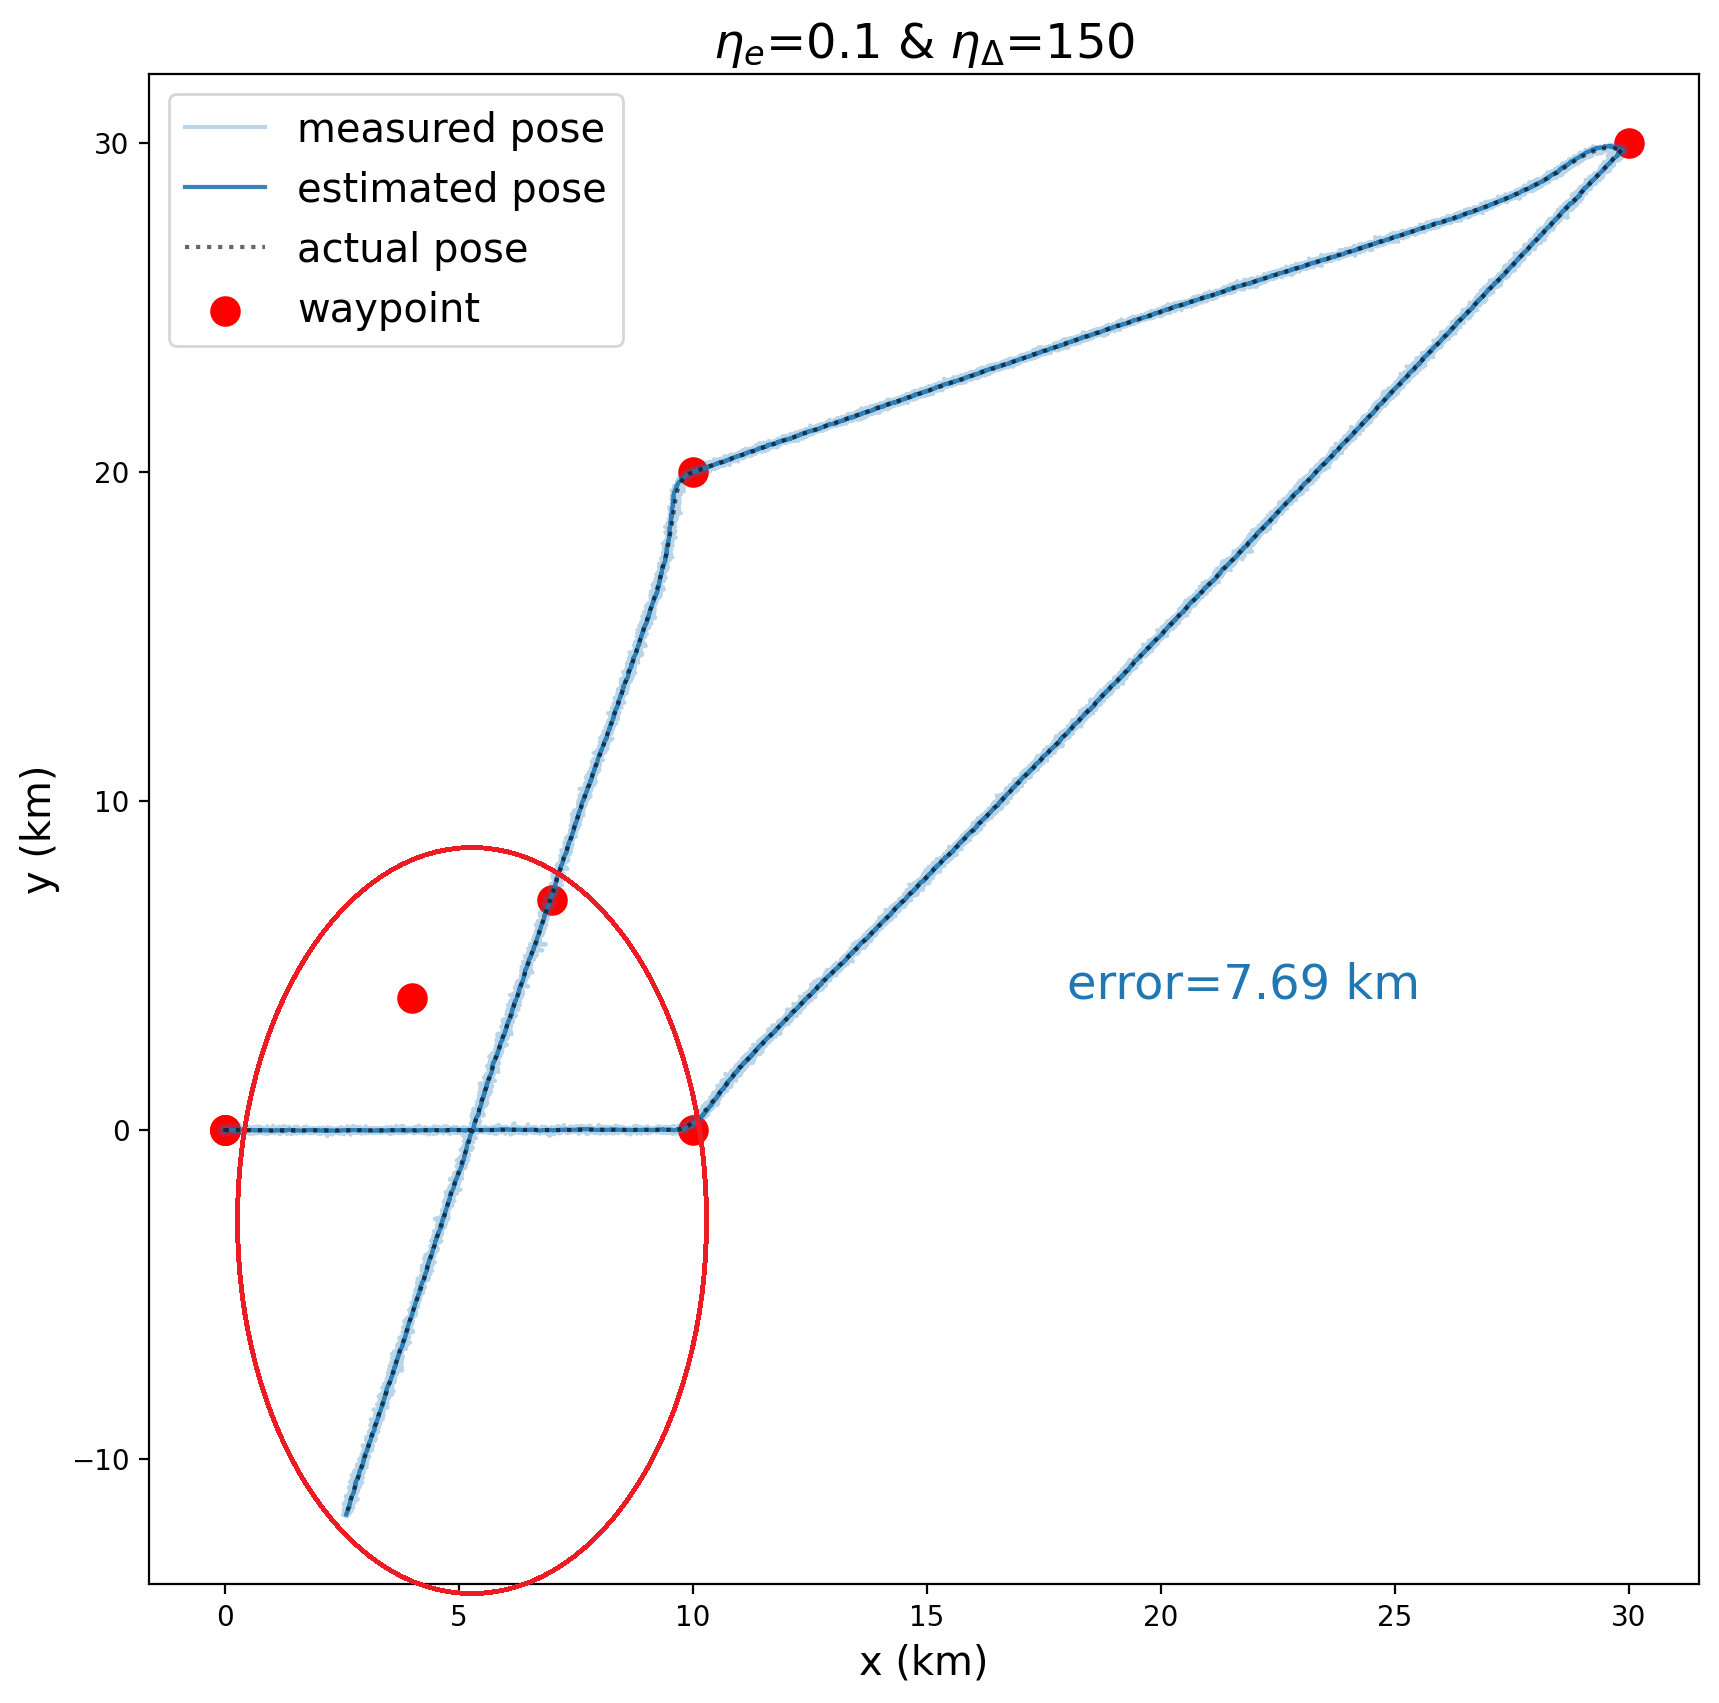
\includegraphics[width=\linewidth]{figures/lookahead_eta_01_150_2d.png}
		\caption{$\eta_e=0.1\:\&\:\eta_\Delta=150$}
	\end{subfigure} 
	\hfill
	\begin{subfigure}[t]{0.24\textwidth}
		\centering
		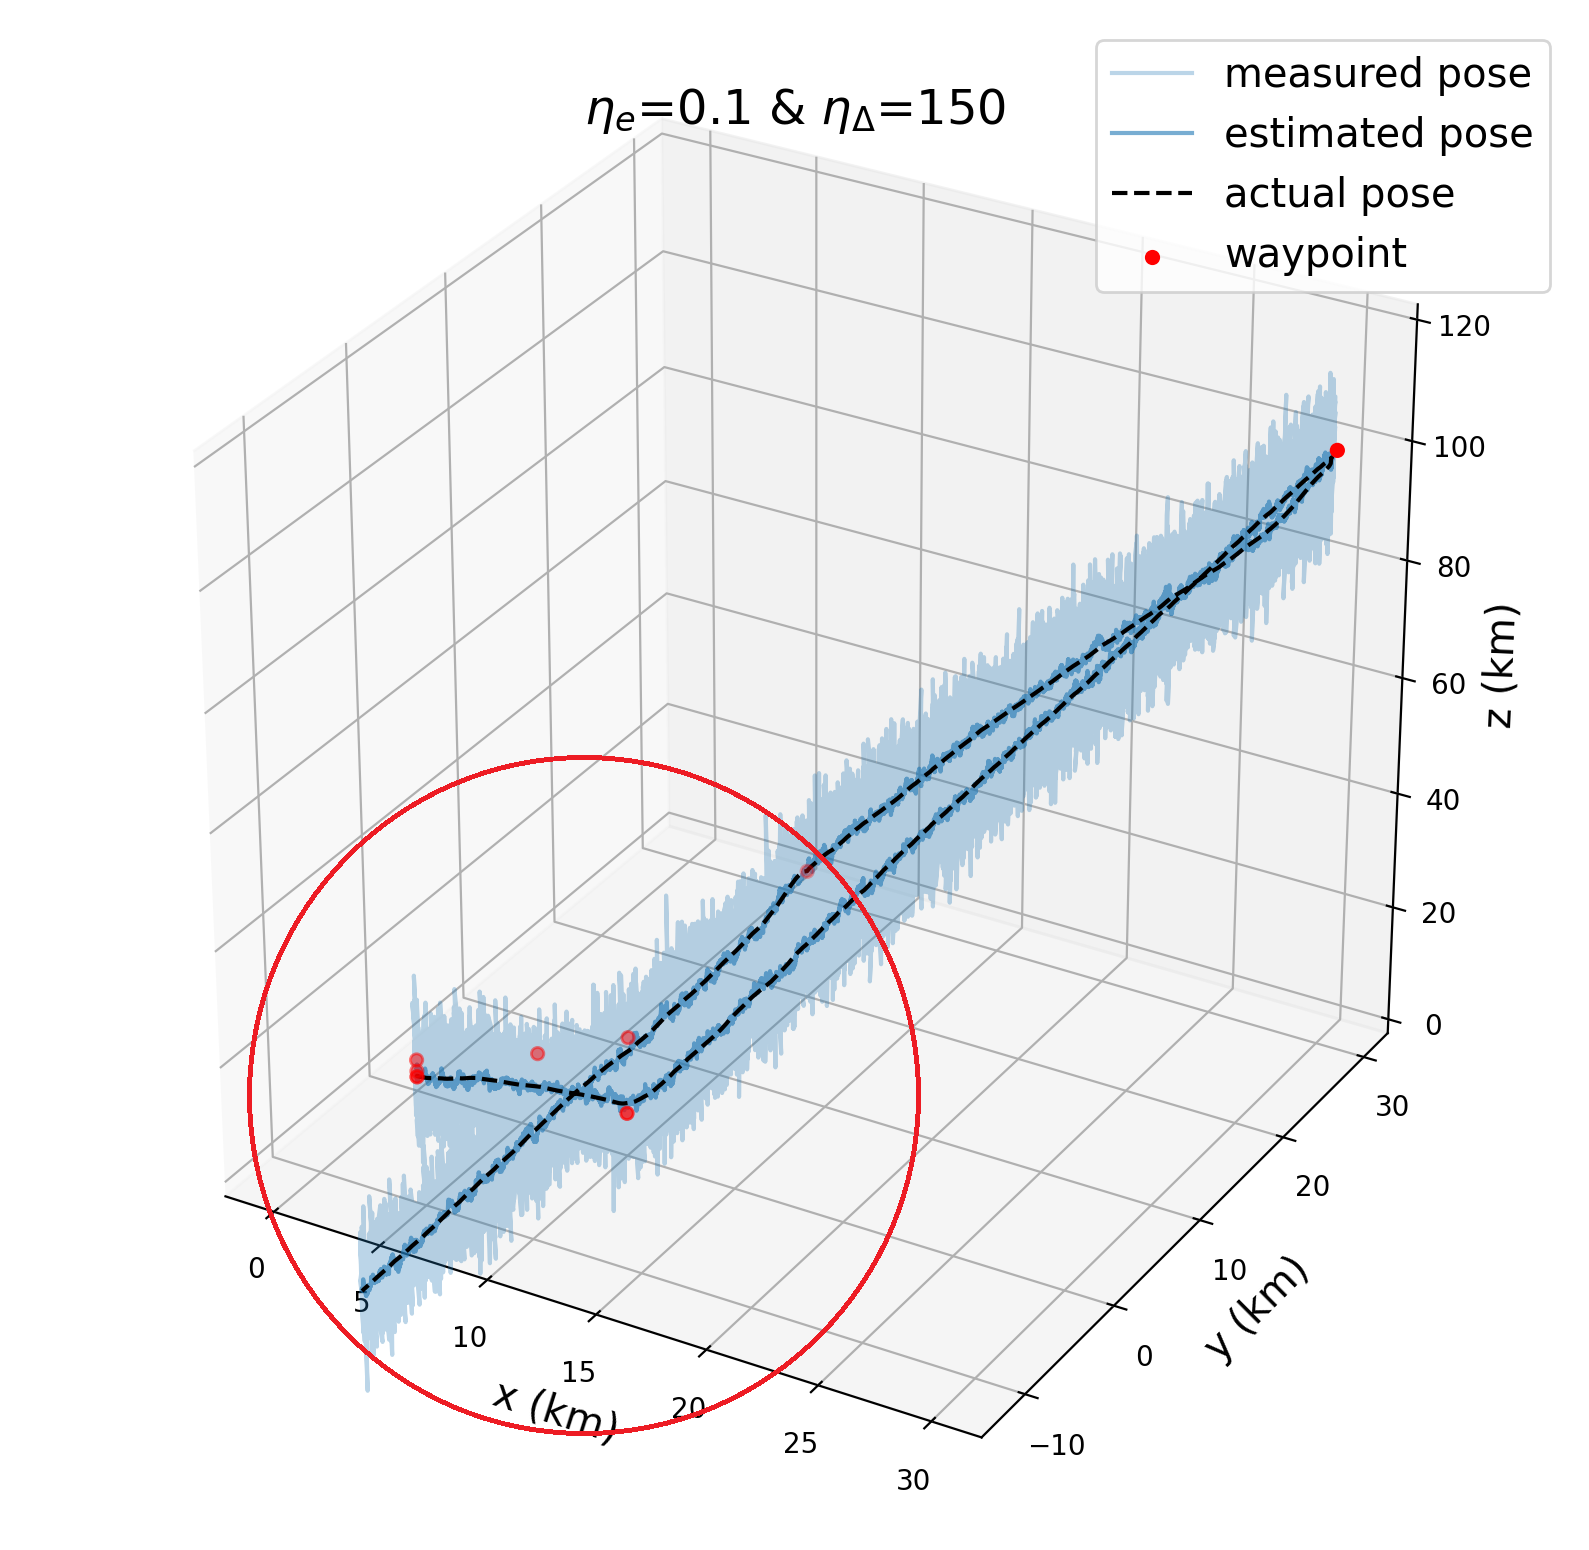
\includegraphics[width=\linewidth]{figures/lookahead_eta_01_150_3d.png}
		\caption{$\eta_e=0.1\:\&\:\eta_\Delta=150$}
	\end{subfigure} \\
	\hfill
	\begin{subfigure}[t]{0.24\textwidth}
		\centering
		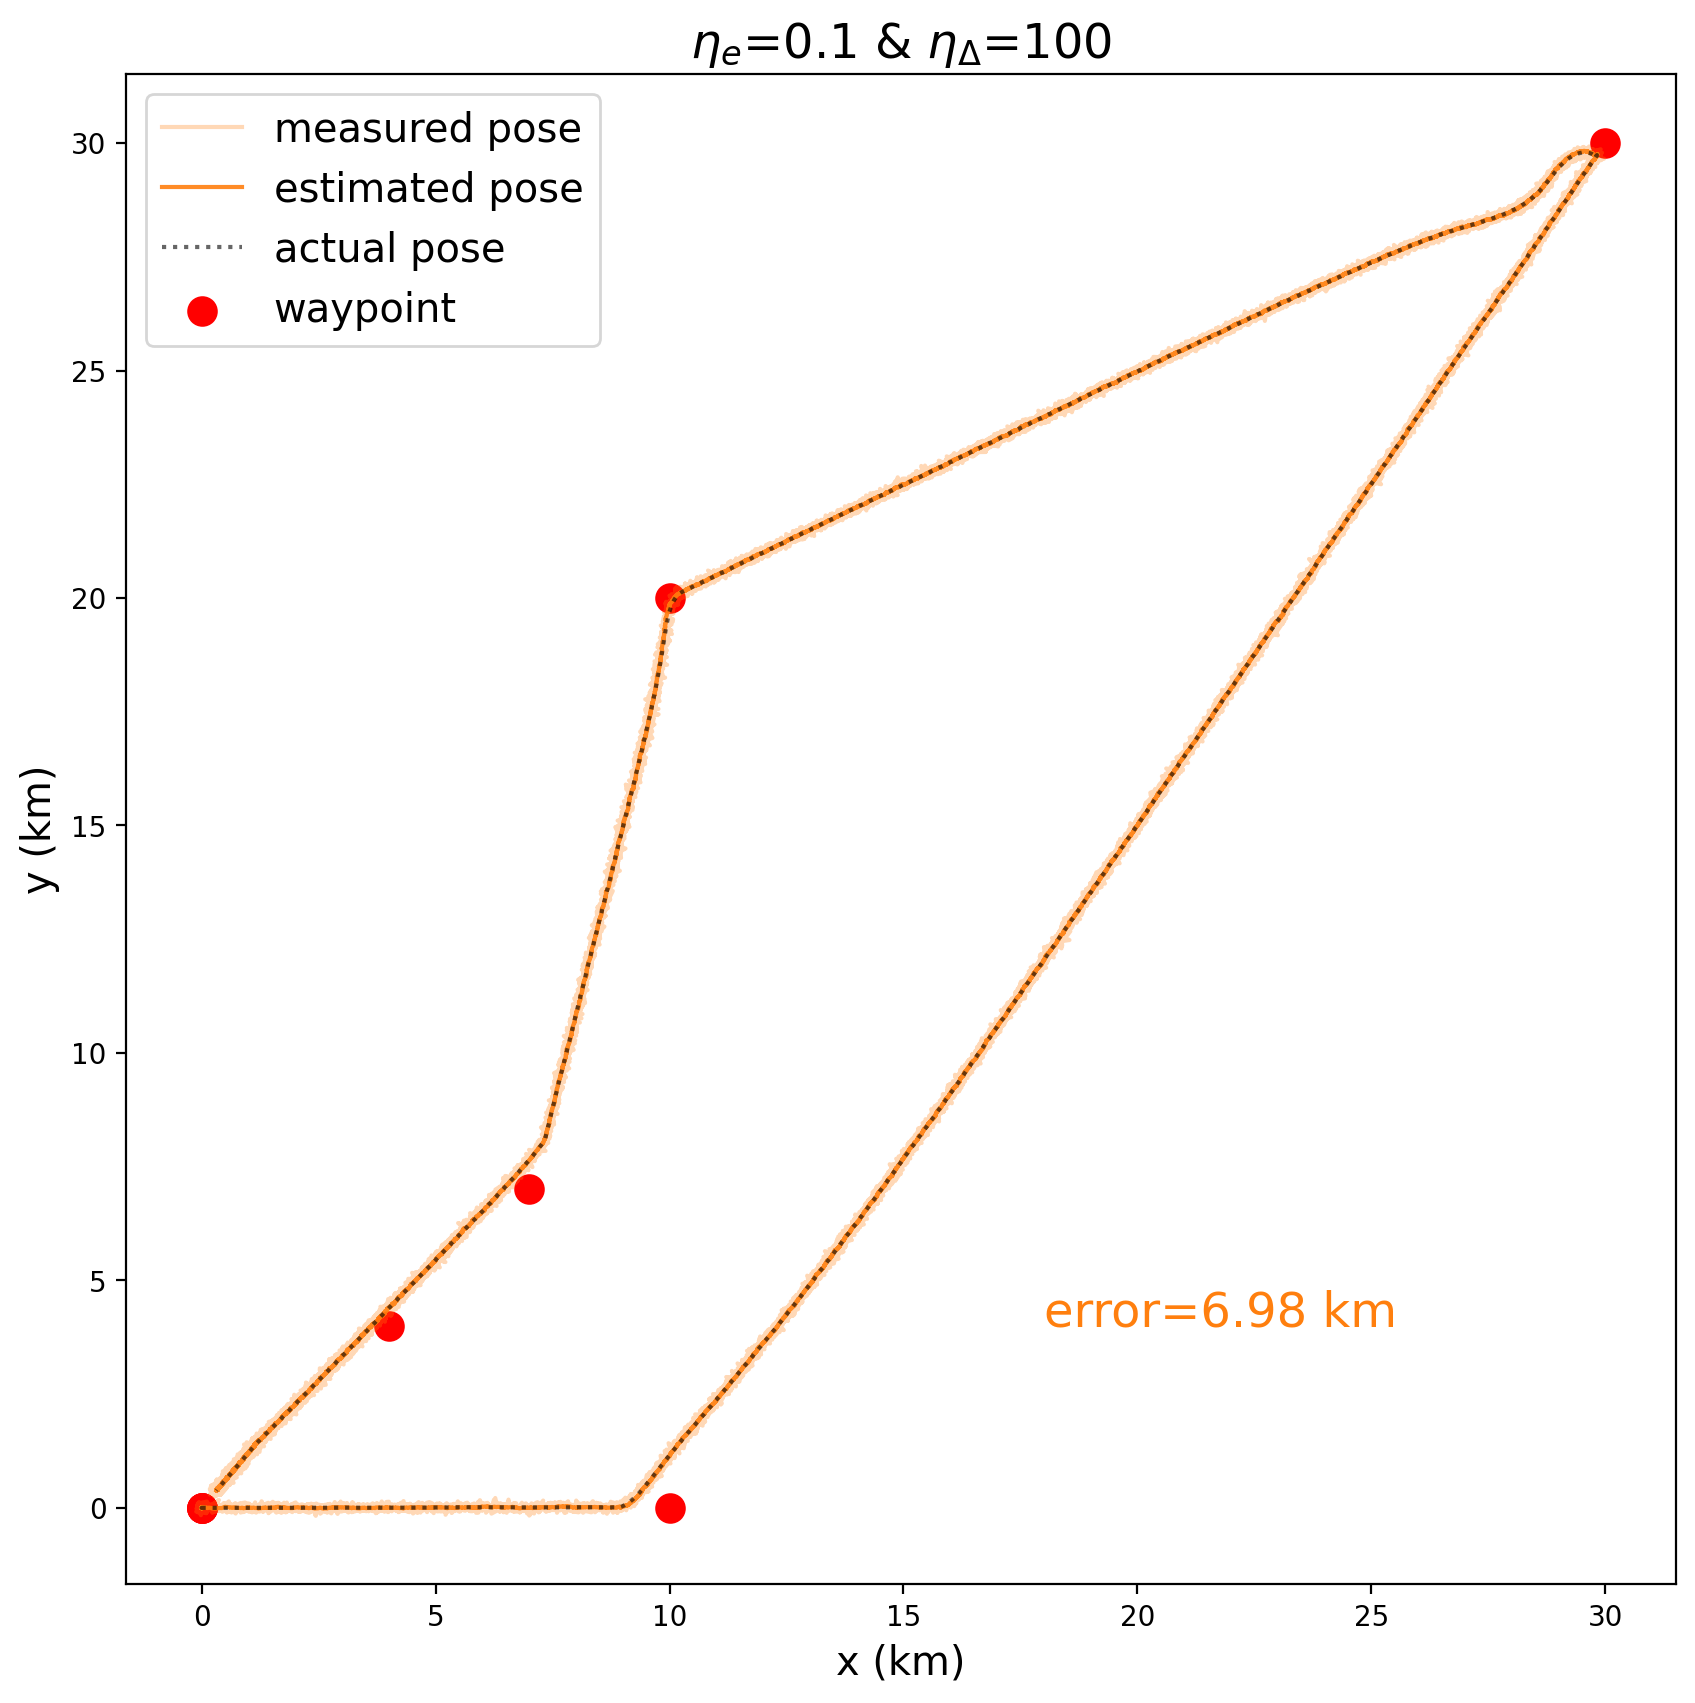
\includegraphics[width=\linewidth]{figures/lookahead_eta_01_100_2d.png}
		\caption{$\eta_e=0.1\:\&\:\eta_\Delta=100$}
	\end{subfigure} 
	\hfill
	\begin{subfigure}[t]{0.24\textwidth}
		\centering
		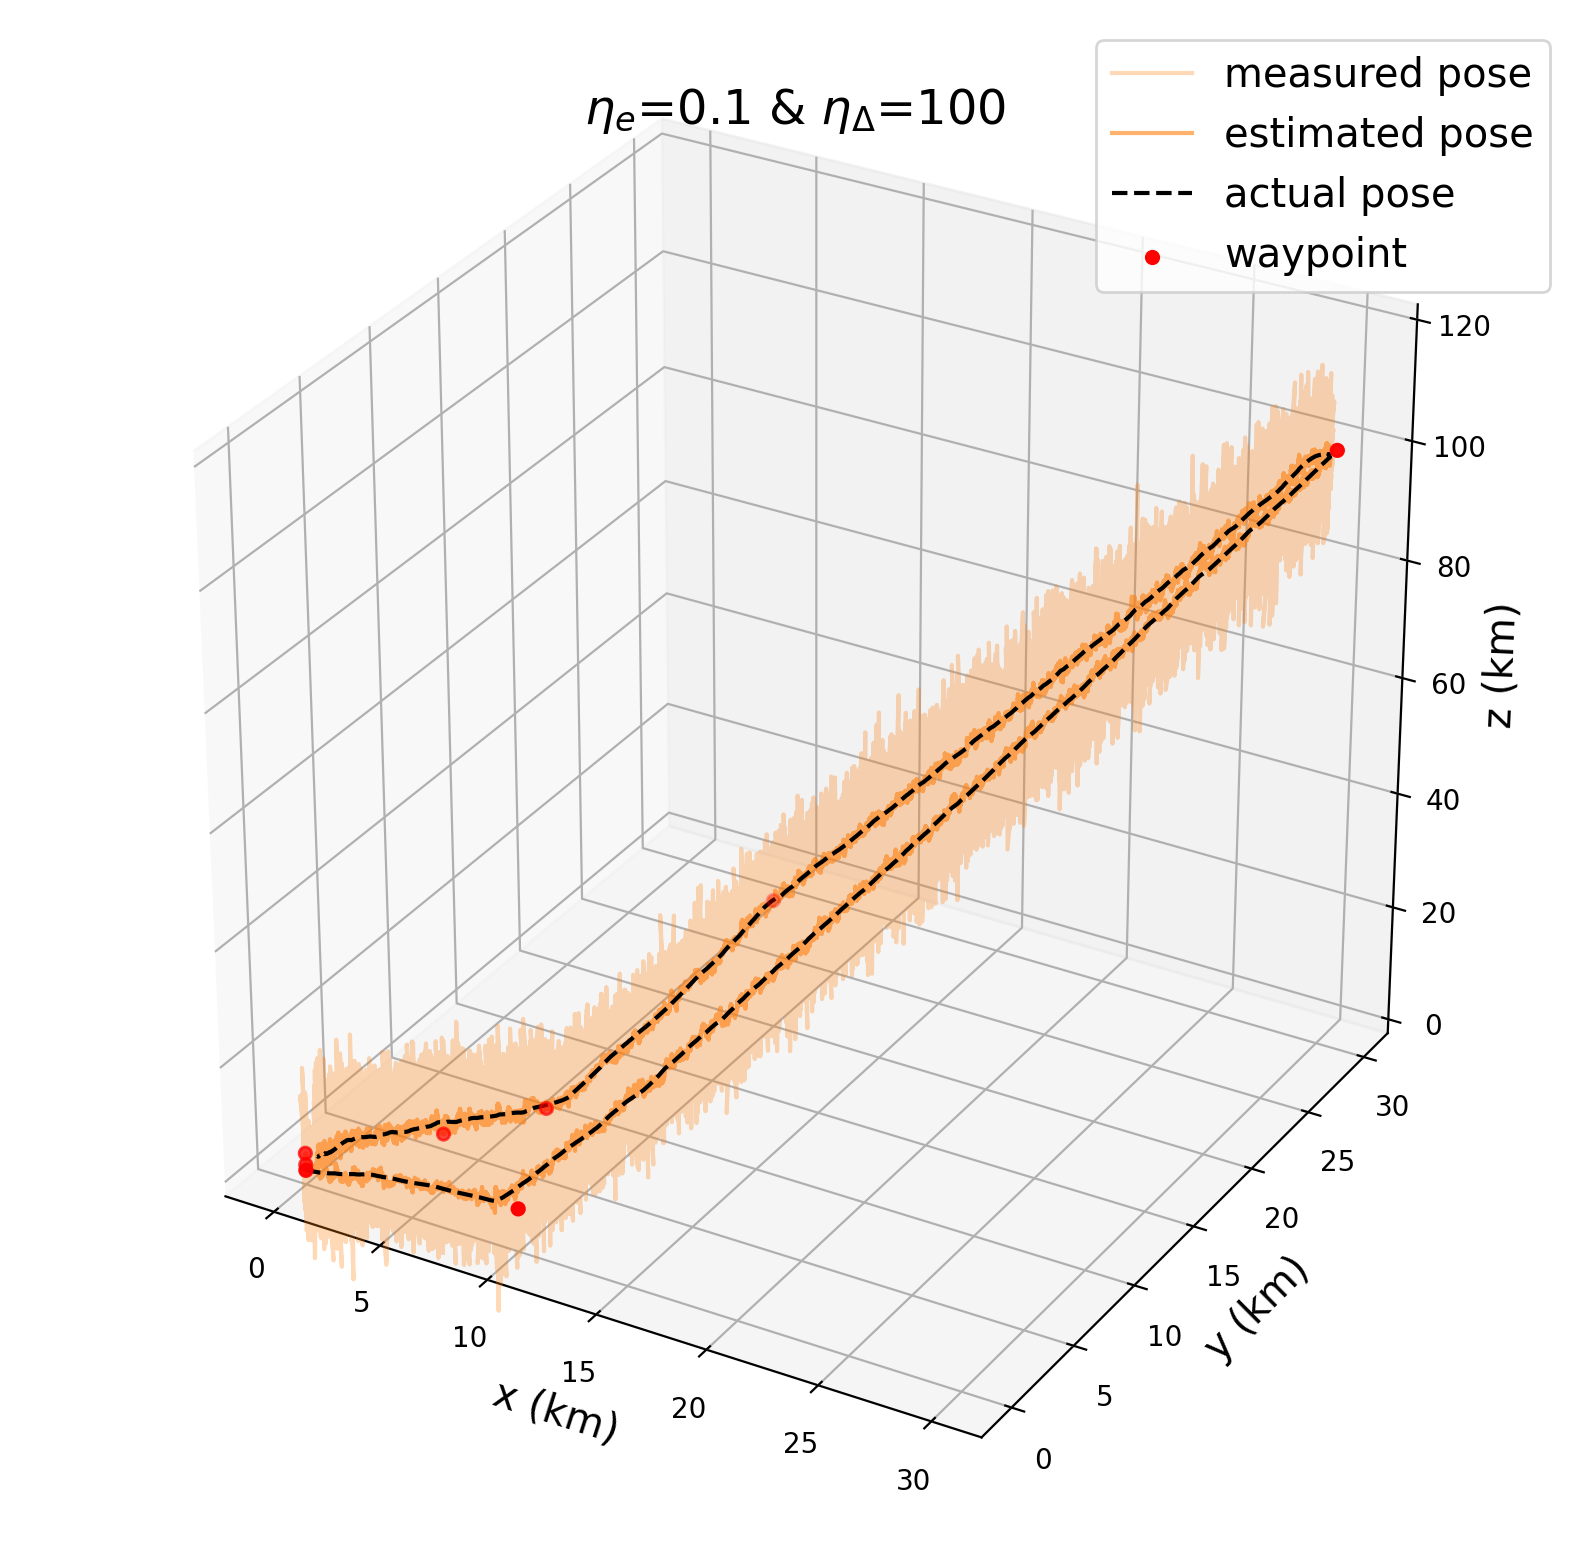
\includegraphics[width=\linewidth]{figures/lookahead_eta_01_100_3d.png}
		\caption{$\eta_e=0.1\:\&\:\eta_\Delta=100$}
	\end{subfigure} \\
	\hfill
	\begin{subfigure}[t]{0.24\textwidth}
		\centering
		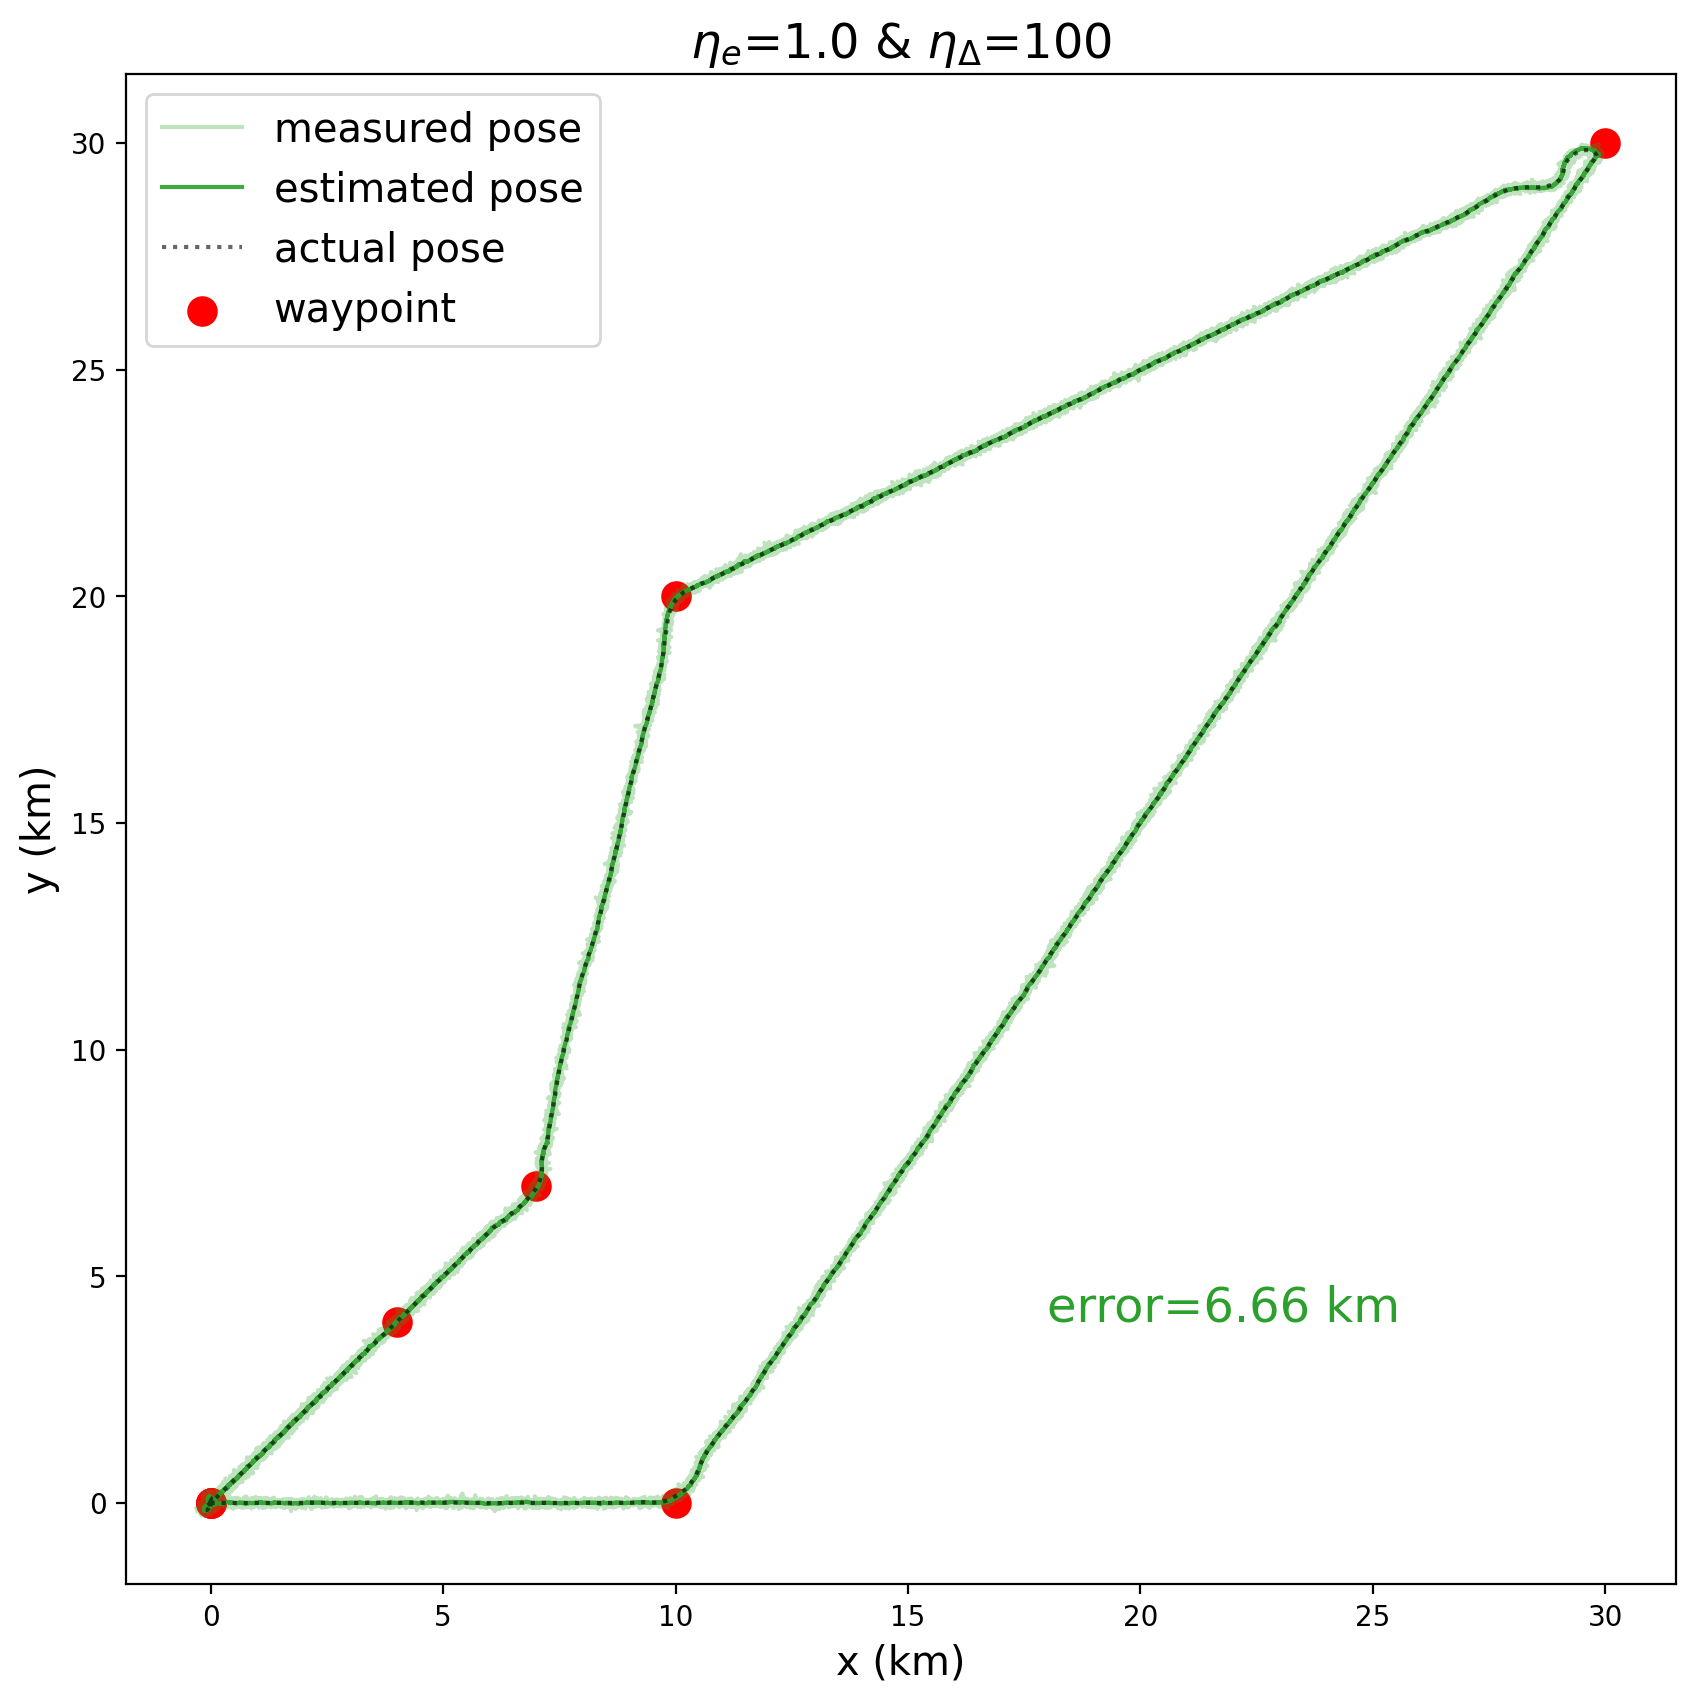
\includegraphics[width=\linewidth]{figures/lookahead_eta_10_100_2d.png}
		\caption{$\eta_e=1.0\:\&\:\eta_\Delta=100$}
	\end{subfigure} 
	\hfill
	\begin{subfigure}[t]{0.24\textwidth}
		\centering
		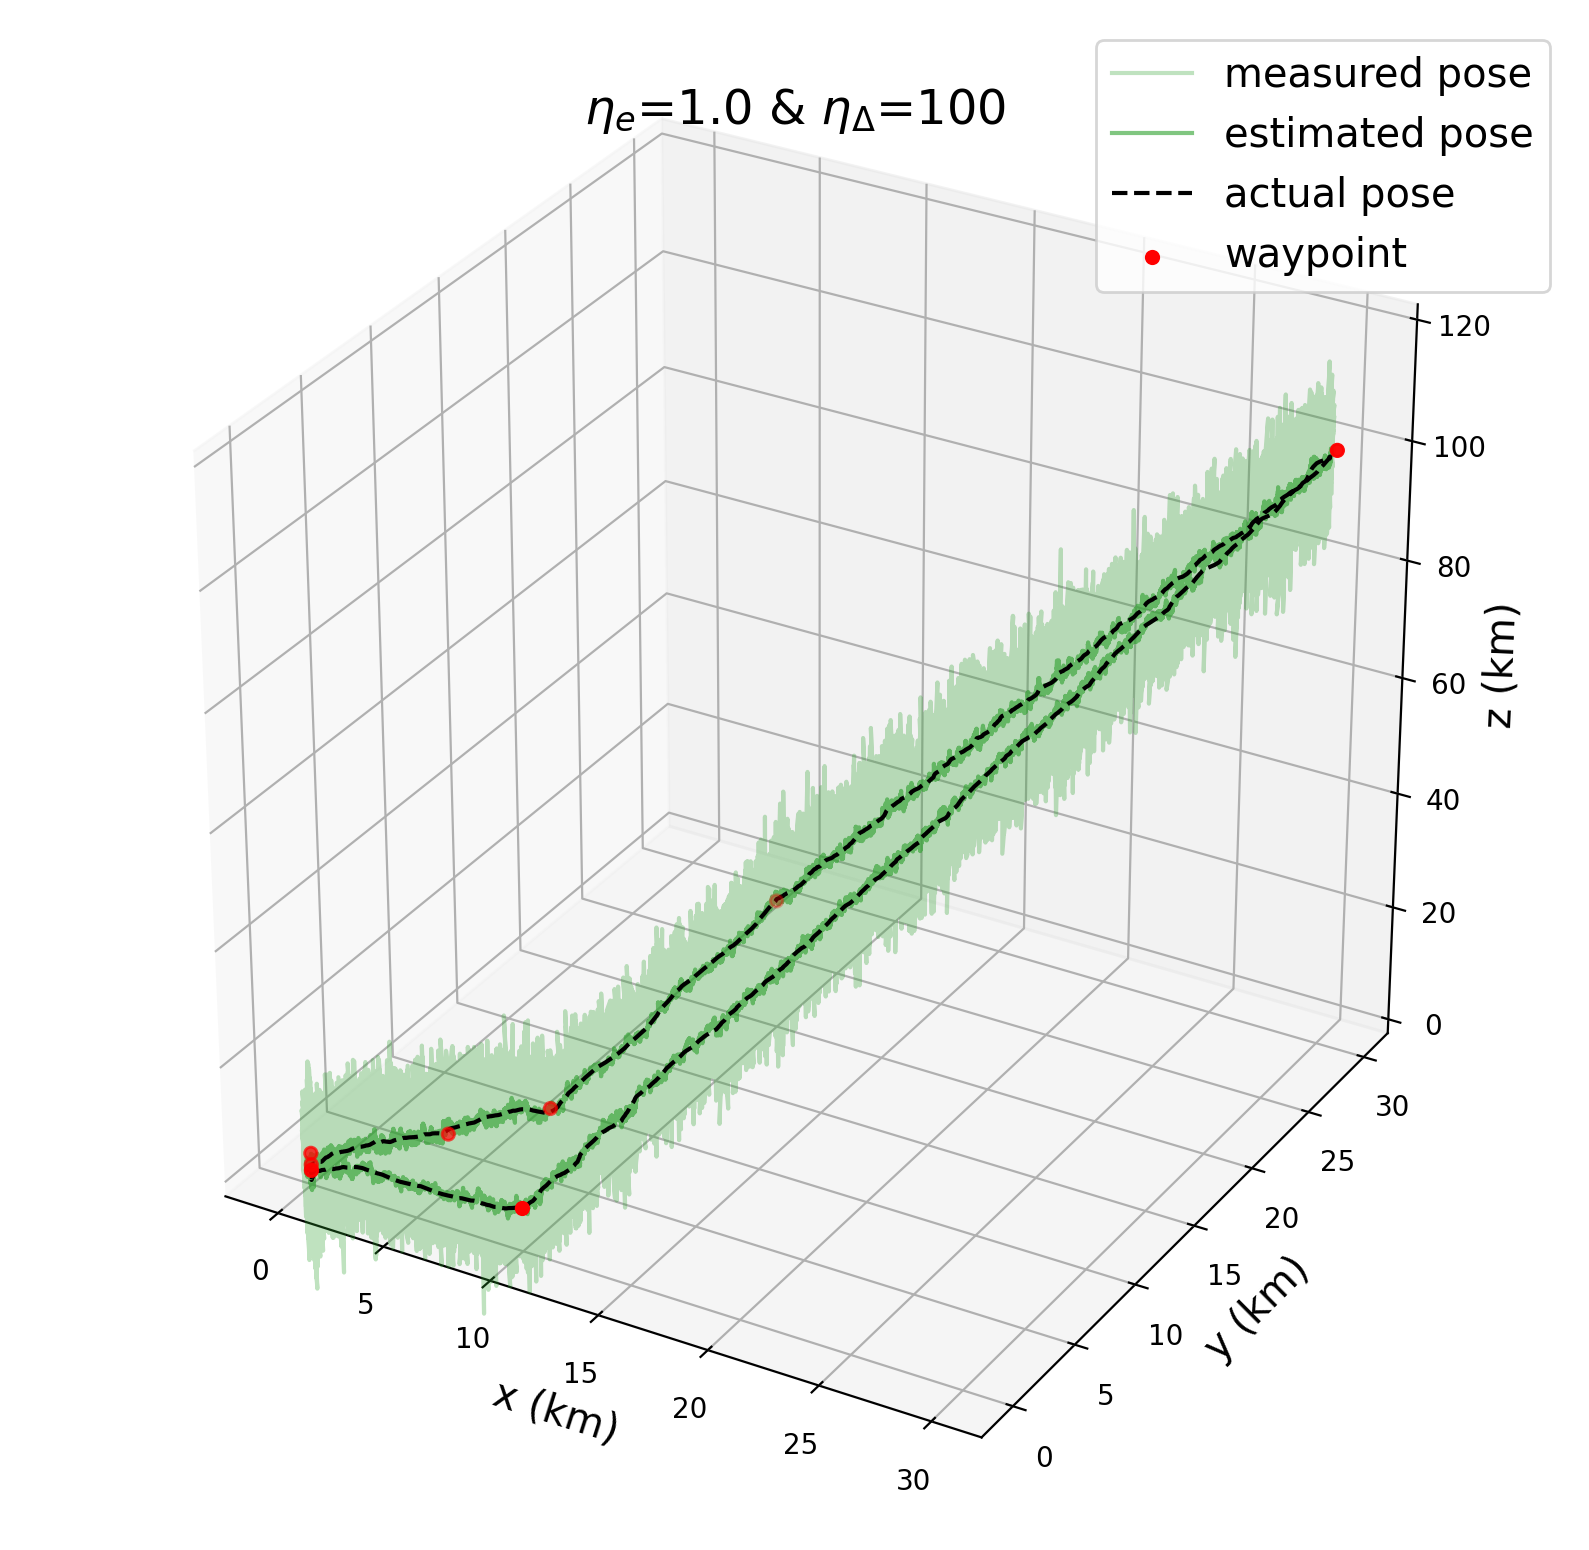
\includegraphics[width=\linewidth]{figures/lookahead_eta_10_100_3d.png}
		\caption{$\eta_e=1.0\:\&\:\eta_\Delta=100$}
	\end{subfigure} \\
	\hfill
	\begin{subfigure}[t]{0.24\textwidth}
		\centering
		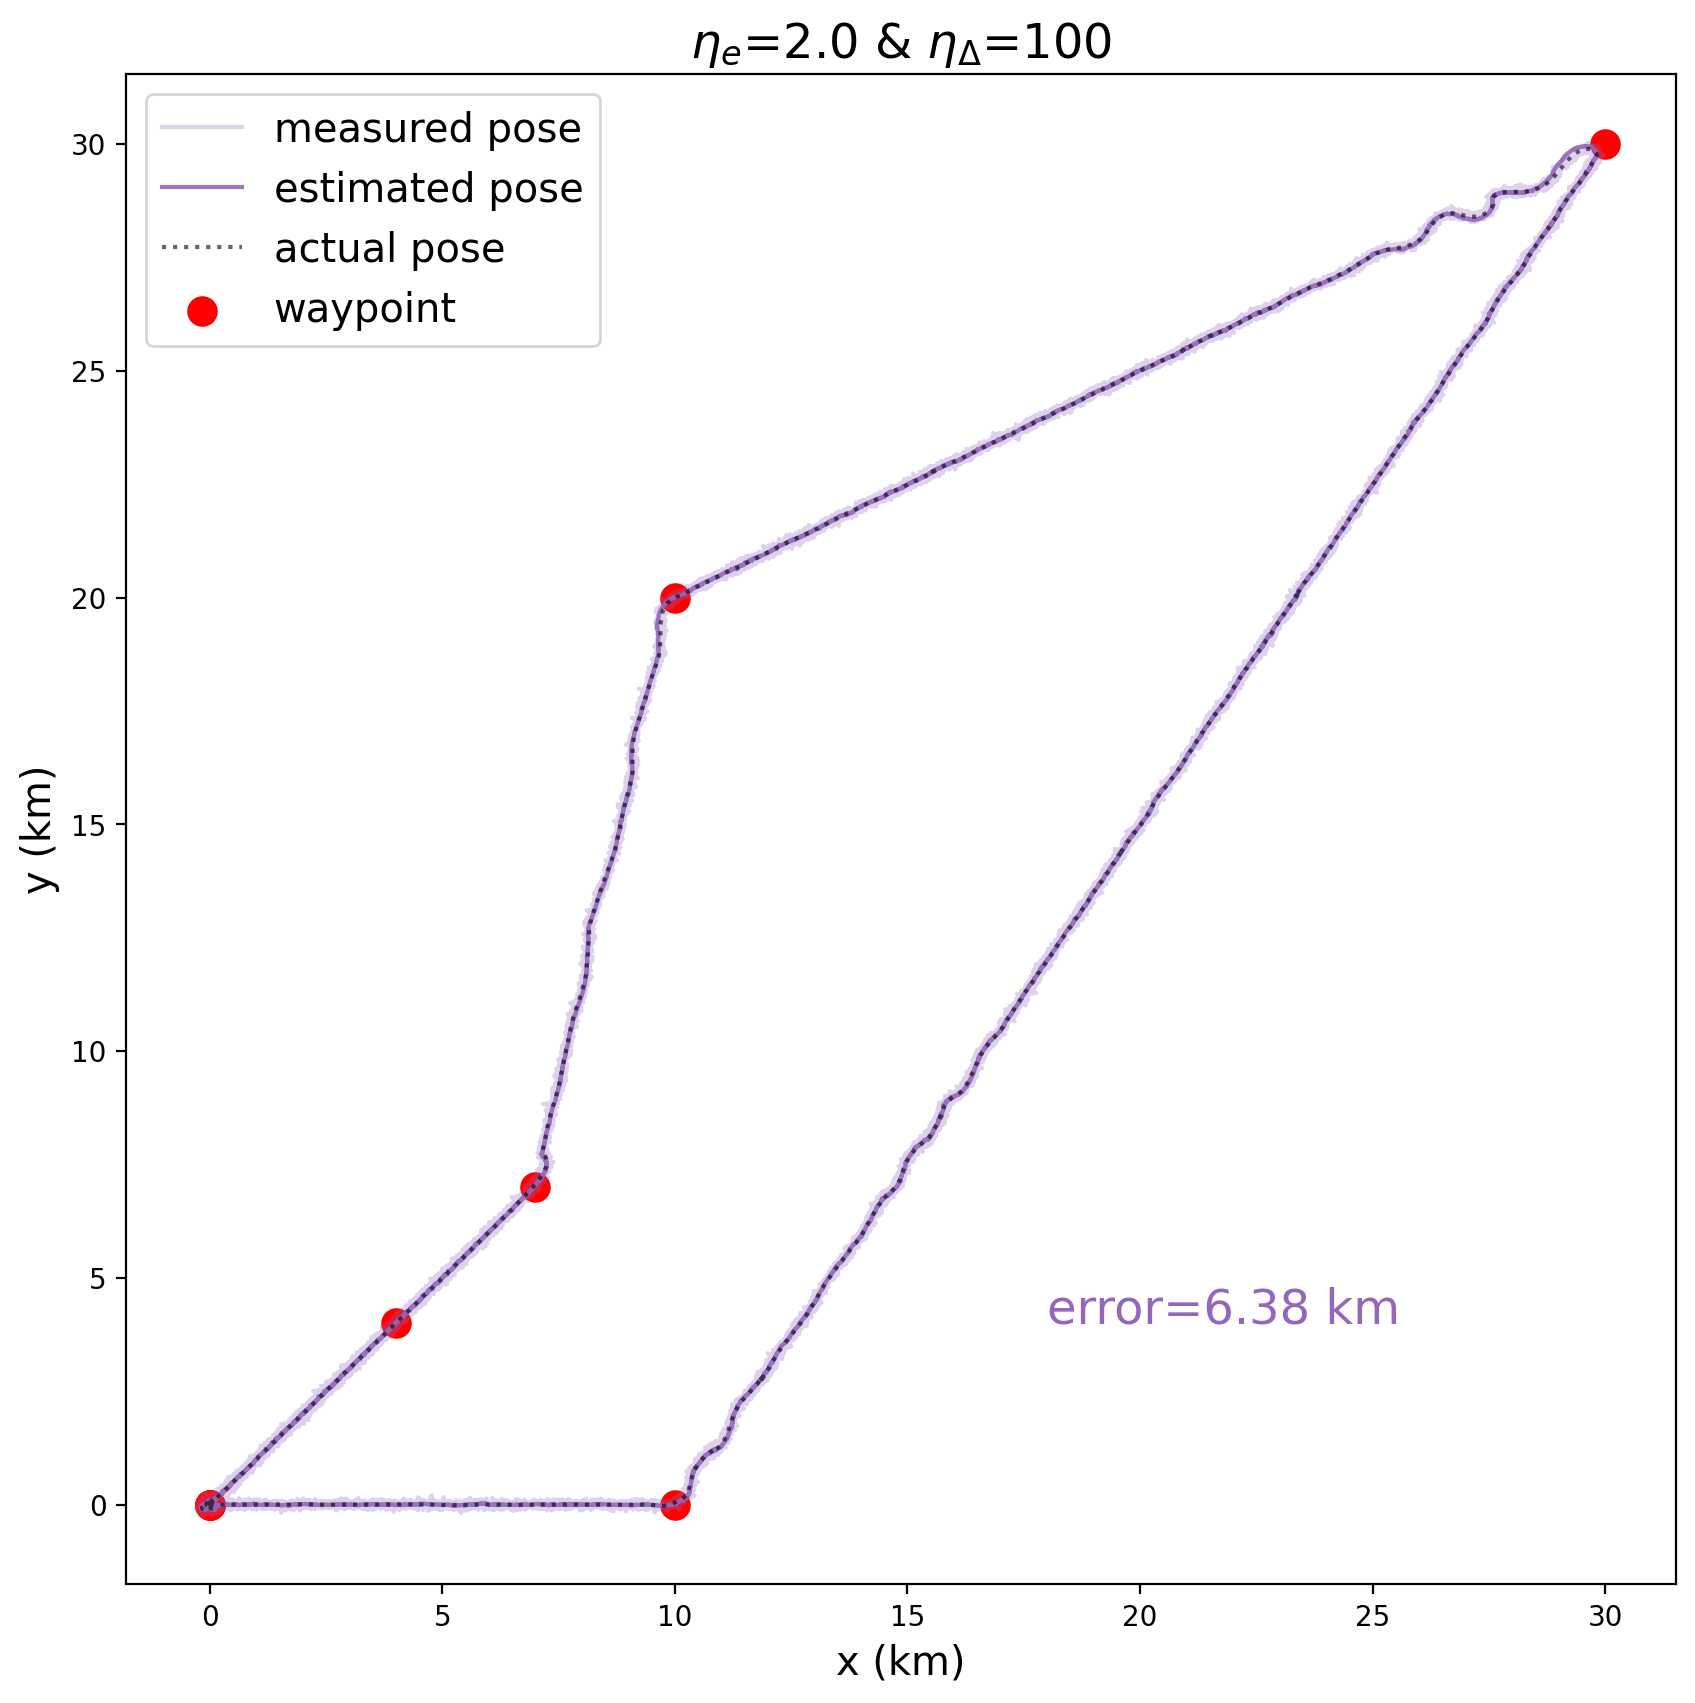
\includegraphics[width=\linewidth]{figures/lookahead_eta_20_100_2d.png}
		\caption{$\eta_e=2.0\:\&\:\eta_\Delta=100$}
	\end{subfigure} 
	\hfill
	\begin{subfigure}[t]{0.24\textwidth}
		\centering
		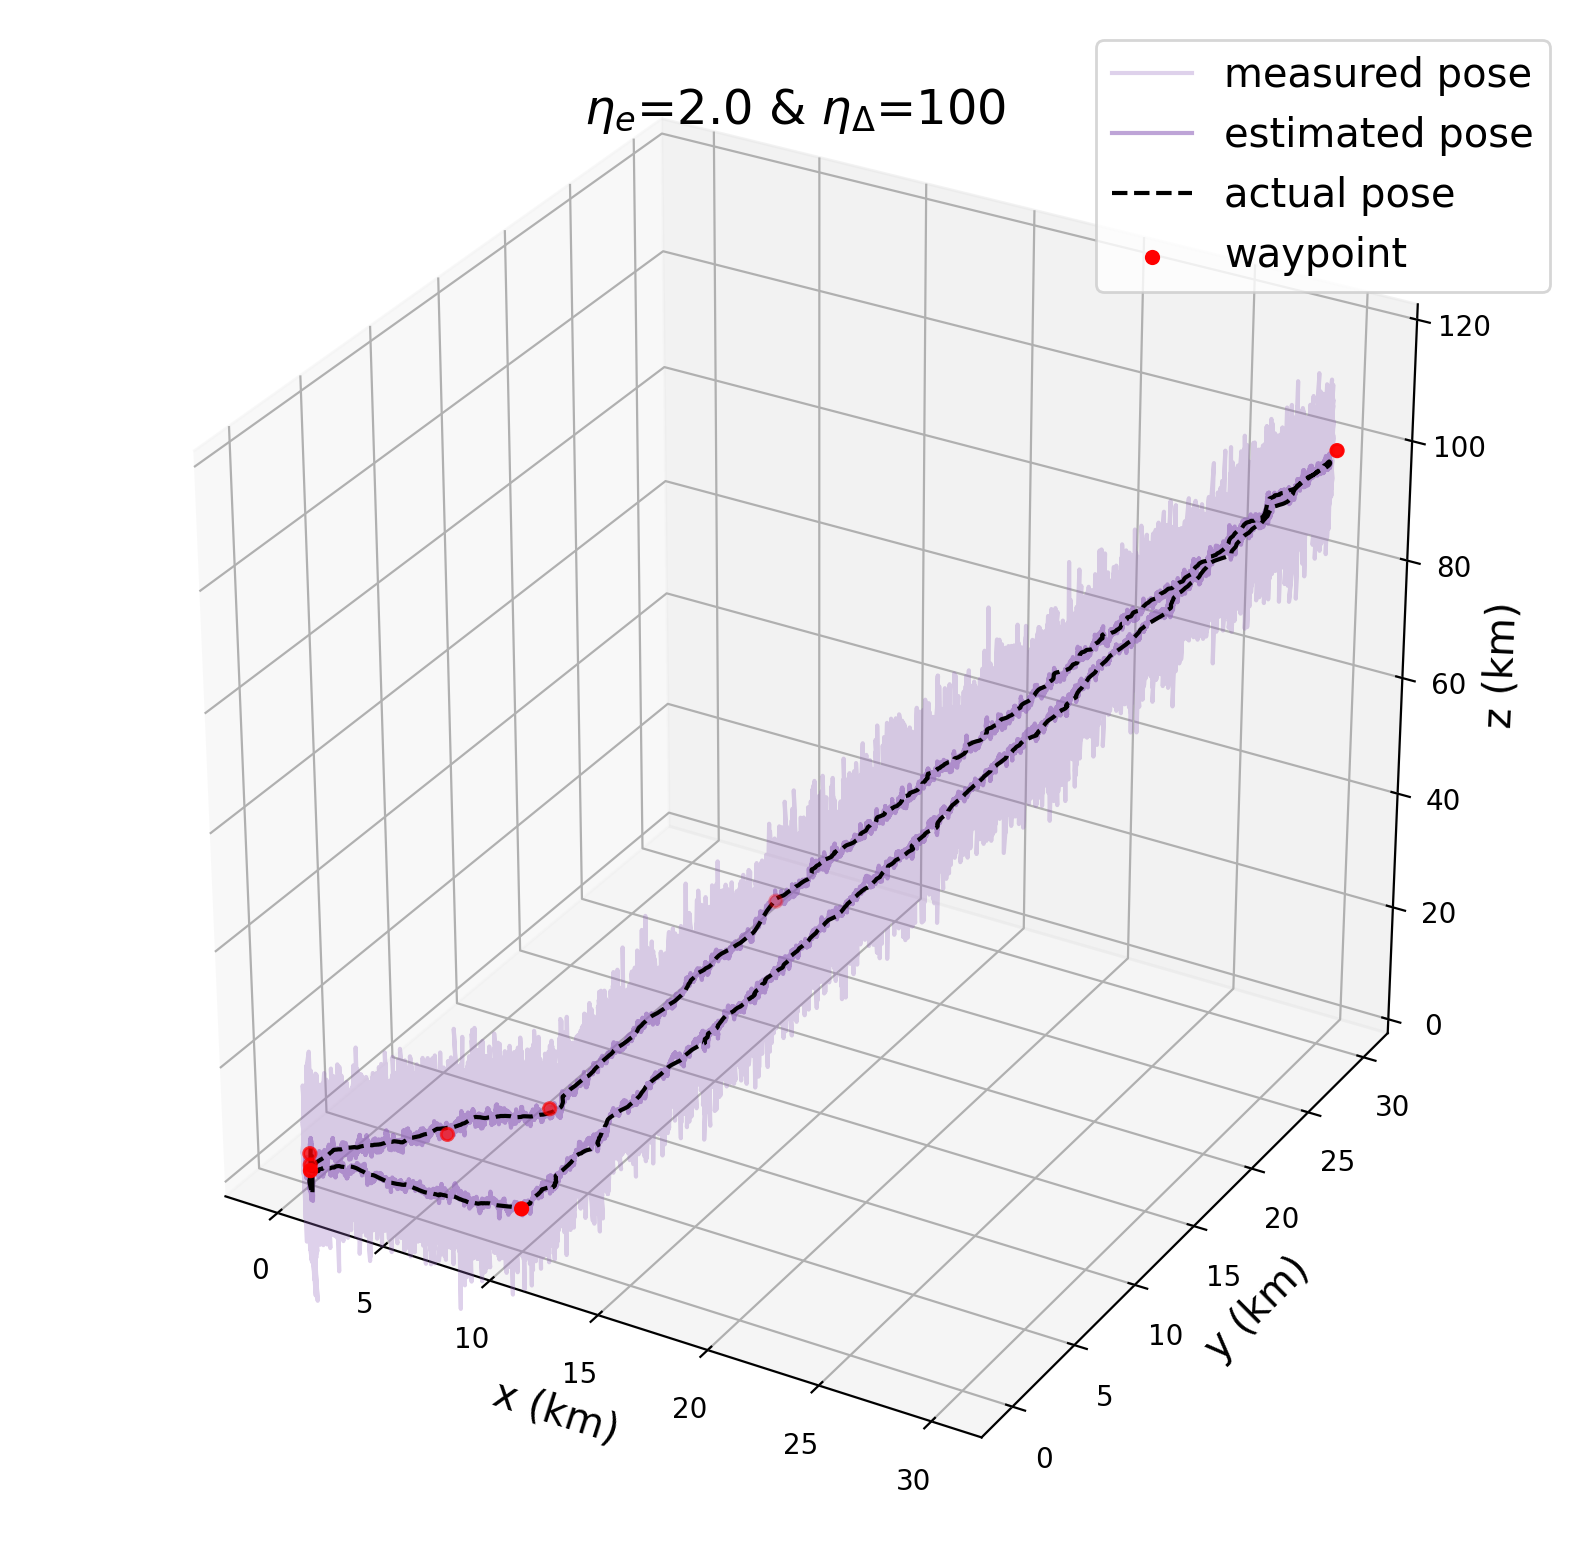
\includegraphics[width=\linewidth]{figures/lookahead_eta_20_100_3d.png}
		\caption{$\eta_e=2.0\:\&\:\eta_\Delta=100$}
	\end{subfigure} 
	
	\caption{Two-dimensional plot (left column: a, c, e, and g) and three-dimensional plot (right column: b, d, f and h) of the measured trajectories and the estimated trajectories with $\eta_e=0.1\:\&\:\eta_\Delta=150$ (blue), $\eta_e=0.1\:\&\:\eta_\Delta=100$ (orange), $\eta_e=1.0\:\&\:\eta_\Delta=100$ (green), and $\eta_e=2.0\:\&\:\eta_\Delta=100$ (purple).}
	\label{fig:exp_lookahead}
\end{figure}

 The result of the third experiment is shown in Fig.~\ref{fig:exp_lookahead}. The figure presents that, changing increasing $\eta_e$ improves the response of the system, while increasing $\eta_\Delta$ disable the spaceship to move between close waypoints. Setting $\eta_\Delta$ to 100 seems to be an optimal point. If we increase it beyond this, the x-wing fighter will lose the ability to reach the next waypoint that locates close to the previous one. The spaceship might be unable to reach the acceptance sphere as highlighted by the red circles in Fig.~\ref{fig:exp_lookahead}(a,b). This is because, the lookahead distance go over the next waypoint, and the x-wing fighter's guidance system cannot see it. $\eta_e$ has a significant effect in reducing the root-mean-square error between the trajectory and the expected linear segment between waypoints. The error drops from 6.98 km to 6.66 km if $\eta_e=1.0$ and to 6.38 km if $\eta_e=2.0$. Setting this value to high can causes multiple oscillation even if the spaceship perfectly stays on a strength path for a while, as shown in Fig.~\ref{fig:exp_lookahead}(g,h). 
 
 The most appropriate set of parameters is found to be $\lambda_Q=1$, $:\lambda_R=1,000$, $K_p=1,000$ $K_d=1,500$, $\eta_e=1.0$, and $\eta_\Delta=100$. With this set of parameters, the autonomous x-wing fighter is simulated, and the video is available at \href{https://youtu.be/vUd8cK0Ot9s}{\url{https://youtu.be/vUd8cK0Ot9s}}.

\begin{figure}[!h]
	\centering
	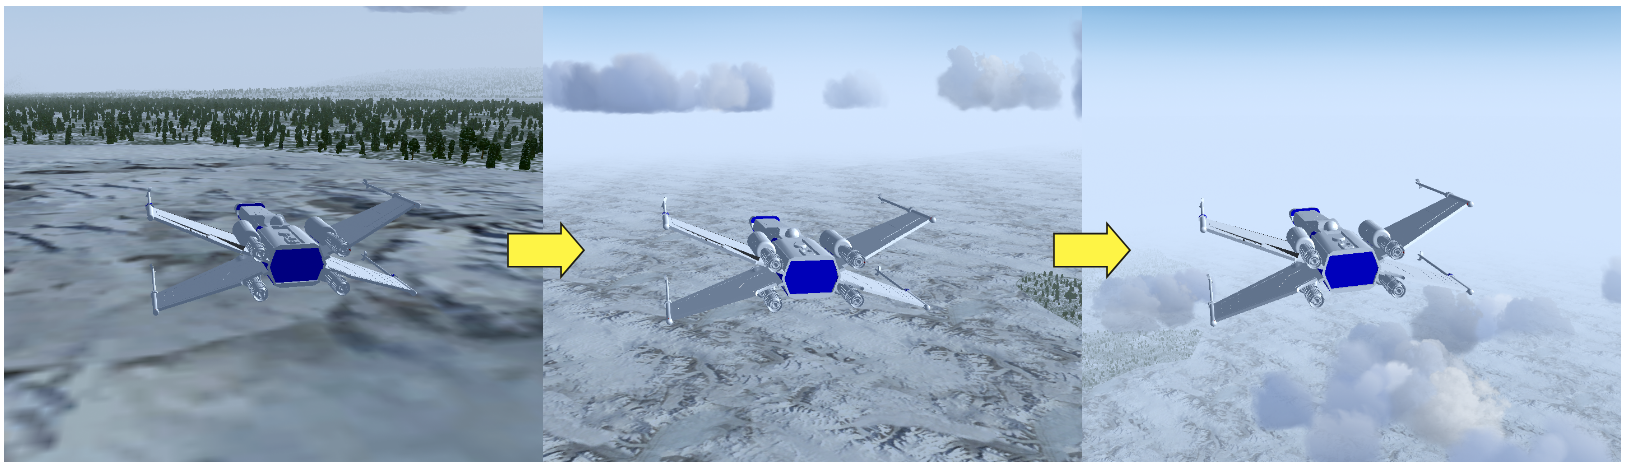
\includegraphics[width=1.0\linewidth]{figures/screenshots}
	\caption{Screenshots from the demonstration video. The video is available at \href{https://youtu.be/vUd8cK0Ot9s}{\url{https://youtu.be/vUd8cK0Ot9s}}.}
	\label{fig:screenshot}
\end{figure}

